\documentclass[11pt]{article}

% ---------------------------------------------------------------------------
%  Mathematical and physical foundations of the KT-D1V5 finite-volume
%  discrete Boltzmann solver (generalized-minmod MUSCL + SSP-RK3)
%  Build:  tectonic d1v5_solver_mathematics.tex
% ---------------------------------------------------------------------------

\usepackage[letterpaper,margin=1in]{geometry}
\usepackage[T1]{fontenc}
\usepackage{lmodern}
\usepackage{microtype}
\usepackage{amsmath,amssymb,amsthm,bm,mathtools}
\usepackage{graphicx}
\usepackage{booktabs,array,multirow,tabularx}
\usepackage{xcolor}
\usepackage{caption,subcaption}
\usepackage{enumitem}
\usepackage{algorithm}
\usepackage{algpseudocode}
\usepackage{tikz}
\usetikzlibrary{arrows.meta,calc,positioning,decorations.pathreplacing}
\usepackage[numbers,sort&compress]{natbib}
\usepackage[colorlinks=true,linkcolor=blue!50!black,citecolor=blue!50!black,urlcolor=blue!50!black]{hyperref}
\usepackage{cleveref}
\usepackage{xurl}
\newcommand{\file}[1]{\nolinkurl{#1}}

\captionsetup{font=small,labelfont=bf}
\setlist{itemsep=2pt,topsep=4pt}
\graphicspath{{figures/}}

\newtheorem{proposition}{Proposition}
\theoremstyle{remark}
\newtheorem{remark}{Remark}

\newcommand{\feq}{f^{\mathrm{eq}}}
\newcommand{\dd}{\mathrm{d}}
\newcommand{\pd}[2]{\frac{\partial #1}{\partial #2}}
\newcommand{\Kn}{\mathrm{Kn}}
\newcommand{\ord}{\mathcal{O}}
\newcommand{\minmod}{\operatorname{minmod}}
\makeatletter
\newcommand{\tabinput}[1]{\@@input #1 }  % primitive input: safe inside tabular
\makeatother

% auto-generated by make_results_figures.m
\newcommand{\contactWidthSlope}{0.73}
\newcommand{\shockWidthSlope}{0.98}
\newcommand{\kinContactMin}{1.2\times10^{-3}}
\newcommand{\kinContactMax}{1.5\times10^{-3}}
\newcommand{\rhoFloorMin}{3.7\times10^{-4}}
\newcommand{\rhoFloorMax}{4.2\times10^{-4}}
\newcommand{\fitLtwoA}{0.490}
\newcommand{\fitLtwoB}{0.458}
\newcommand{\fitLtwoC}{0.634}
\newcommand{\fitLtwoD}{0.403}
\newcommand{\fitLtwoAvgA}{0.482}
\newcommand{\fitLtwoAvgB}{0.347}
\newcommand{\fitLtwoAvgC}{0.614}
\newcommand{\fitLtwoAvgD}{0.358}
\newcommand{\shockPhaseSlopeA}{0.498}
\newcommand{\shockPhaseSlopeB}{0.513}
\newcommand{\zoneSlopeAA}{0.77}
\newcommand{\zoneSlopeAB}{0.41}
\newcommand{\zoneSlopeAC}{0.58}
\newcommand{\zoneSlopeDA}{0.76}
\newcommand{\zoneSlopeDB}{0.38}
\newcommand{\zoneSlopeDC}{0.47}


\title{\textbf{Mathematical and Physical Foundations of the\\ KT-D1V5 Finite-Volume Discrete Boltzmann Solver}\\[4pt]
\large MUSCL reconstruction with a generalized-minmod limiter, SSP-RK3 time integration,\\ and the Sod shock-tube benchmark}
\author{Nathan Kidwell\\ \small Compressible-flow DBM research, Embry-Riddle Aeronautical University}
\date{September 18, 2026}

\begin{document}
\maketitle

\begin{abstract}
\noindent
This report explains, without reference to code, the mathematics and physics that
underlie the one-dimensional finite-volume discrete Boltzmann solver
\file{d1v5_sodshock_muscl_MC_RK3.m}.
The solver advances five discrete velocity populations of the Kataoka--Tsutahara
(KT) D1V5 model under a Bhatnagar--Gross--Krook (BGK) relaxation, transports them
with an upwind finite-volume flux built on a MUSCL reconstruction limited by the
generalized-minmod slope ($\theta = 1.2$), and integrates in time with the
three-stage strong-stability-preserving Runge--Kutta method.
Each ingredient is derived from first principles: the moment system that fixes the
equilibrium, the inverse map from populations to density, velocity, temperature
and pressure, the Chapman--Enskog expansion of the discrete model, the exact
Riemann solution of the Sod problem, total-variation-diminishing (TVD) limiter
theory, the stability of the time integrator, and the error norms used for
validation.
The analysis yields several results that are specific to this model and were
checked numerically: the D1V5 model reproduces the Euler equations exactly at
leading order, but its $\ord(\tau)$ dissipation is \emph{not} Navier--Stokes;
the contact discontinuity diffuses with a velocity-dependent coefficient
$D_c = \tau (v_1^2-U^2)(v_2^2-U^2)/[(b+2)T]$ that vanishes as the flow speed
approaches the slow lattice speed; and the BGK stiffness is exactly $1/\tau$.
A five-grid convergence study ($N_x = 3125$--$50{,}000$, $\tau = 5\times10^{-6}$,
$\mathrm{CFL}=0.025$) together with a matched limiter comparison and a
$\theta$-sweep is reported and interpreted with these results.
\end{abstract}

\tableofcontents
\clearpage

% ===========================================================================
\section{Scope, configuration, and notation}
\label{sec:scope}
% ===========================================================================

The solver computes the classical Sod shock tube~\citep{Sod1978} using a
\emph{finite-volume discrete Boltzmann method} (FVDBM).  It does not evolve the Euler
variables $(\rho,\rho u,E)$ directly.  Instead it evolves five scalar fields
$f_i(x,t)$, one per discrete molecular velocity $c_i$, whose velocity moments are
the Euler variables.  The macroscopic gas dynamics emerges from two mechanisms
acting on the populations:
\begin{enumerate}
  \item \textbf{free streaming}: each $f_i$ is advected at its own constant speed
        $c_i$ (a linear hyperbolic problem), and
  \item \textbf{collisions}: each $f_i$ relaxes toward a local equilibrium
        $\feq_i(\rho,u,T)$ at rate $1/\tau$ (a nonlinear but local source).
\end{enumerate}
Discrete Boltzmann models of this kind are used for compressible flow because the
same populations that reproduce the Euler or Navier--Stokes equations also carry
information about thermodynamic non-equilibrium~\citep{XuZhangZhang2018,Gan2018}.
Finite-volume transport of the populations decouples the velocity lattice from the
spatial mesh, which is what makes unstructured and body-fitted grids
possible~\citep{XuChenCai2021}.
\Cref{tab:config} lists the configuration analysed in this report.
All quantities are nondimensional with the specific gas constant set to one, so
the ideal-gas law reads $p=\rho T$ and the sound speed is $a=\sqrt{\gamma T}$.

\begin{table}[ht]
\centering
\caption{Solver configuration used throughout this report (the live solver and
convergence driver of September 18, 2026).}
\label{tab:config}
\small
\begin{tabular}{@{}lll@{}}
\toprule
Quantity & Symbol & Value \\
\midrule
Specific-heat ratio & $\gamma$ & $1.4$ \\
Degrees-of-freedom parameter & $b = 2/(\gamma-1)$ & $5$ \\
BGK relaxation time & $\tau$ & $5\times10^{-6}$ \\
Discrete speeds & $v_1,\ v_2$ & $1,\ 3$ \\
Internal-energy parameter & $\eta_0$ & $1.75$ \\
Domain, diaphragm & $L_x,\ x_0$ & $20,\ 10$ \\
Final time & $t_{\mathrm{end}}$ & $0.15$ \\
Limiter & generalized minmod & $\theta = 1.20$ \\
Time integrator & SSP-RK3 & $\Delta t=\min(\mathrm{CFL}\,\Delta x/v_2,\ \tau/4)$ \\
CFL number & CFL & $0.025$ \\
Convergence grids & $N_x$ & $3125,\ 6250,\ 12{,}500,\ 25{,}000,\ 50{,}000$ \\
Boundary condition & --- & zero-gradient (transmissive) \\
Positivity repair & --- & off \\
\bottomrule
\end{tabular}
\end{table}

\paragraph{Claim boundary.}
Everything in this report concerns the one-dimensional Sod problem.  The analysis
explains how the method works and what the measured errors mean; it does not
establish grid independence, a formal order of accuracy on a smooth manufactured
solution, or behaviour in two dimensions.

% ===========================================================================
\section{Kinetic theory background}
\label{sec:kinetic}
% ===========================================================================

\subsection{The BGK--Boltzmann equation}

Let $f(x,\xi,\eta,t)$ be a one-dimensional velocity distribution in which $\xi$ is
the molecular velocity along $x$ and $\eta$ collects the remaining
$b-1$ degrees of freedom (the two transverse translational ones and the
rotational ones of a diatomic gas), treated as a single internal variable.  The
Boltzmann equation with the BGK collision model~\citep{BGK1954} is
\begin{equation}
  \pd{f}{t} + \xi\pd{f}{x} = -\frac{1}{\tau}\bigl(f - \feq\bigr),
  \label{eq:bgk}
\end{equation}
where $\tau$ is a relaxation time and $\feq$ is the local Maxwellian that has the
same density, momentum and energy as $f$:
\begin{equation}
  \feq = \frac{\rho}{(2\pi T)^{b/2}}
  \exp\!\left[-\frac{(\xi-u)^2 + \eta^2}{2T}\right].
\end{equation}
The macroscopic fields are velocity moments of $f$,
\begin{equation}
  \rho = \int f\,\dd\Xi,\qquad
  \rho u = \int \xi f\,\dd\Xi,\qquad
  \rho\,(bT + u^2) = \int (\xi^2 + \eta^2) f\,\dd\Xi,
  \label{eq:moments_cont}
\end{equation}
with $\dd\Xi = \dd\xi\,\dd^{b-1}\eta$.  The quantities $\psi \in \{1,\ \xi,\ \tfrac12(\xi^2+\eta^2)\}$
are \emph{collision invariants}: because $\feq$ shares these moments with $f$,
$\int \psi (\feq - f)\,\dd\Xi = 0$, and multiplying~\eqref{eq:bgk} by $\psi$ and
integrating yields exact conservation laws for mass, momentum and total energy
$E = \tfrac12\rho(bT+u^2)$.  The internal energy per unit mass is $e = bT/2$, so
$c_v = b/2$, $c_p = (b+2)/2$ and $\gamma = (b+2)/b$; $b=5$ gives $\gamma=1.4$.

\subsection{Chapman--Enskog expansion and the hydrodynamic limit}
\label{sec:ce_cont}

When $\tau$ is small compared with the macroscopic time scale (small Knudsen
number $\Kn = \tau a/L$), the Chapman--Enskog procedure~\citep{ChapmanCowling1970,Cercignani1988}
expands
\begin{equation}
  f = \feq + \tau f^{(1)} + \tau^2 f^{(2)} + \cdots,\qquad
  \partial_t = \partial_{t_0} + \tau\partial_{t_1} + \cdots .
\end{equation}
At $\ord(1)$ the moment equations are the Euler equations,
\begin{align}
  \partial_t \rho + \partial_x(\rho u) &= 0, \label{eq:euler_mass}\\
  \partial_t (\rho u) + \partial_x(\rho u^2 + p) &= 0, \label{eq:euler_mom}\\
  \partial_t E + \partial_x\bigl[u(E+p)\bigr] &= 0, \qquad E = \frac{p}{\gamma-1}+\frac12\rho u^2 . \label{eq:euler_energy}
\end{align}
At $\ord(\tau)$, $f^{(1)} = -(\partial_{t_0} + \xi\partial_x)\feq$, which adds a
viscous stress and a heat flux.  For the continuous BGK gas with $b$ degrees of
freedom in one-dimensional flow these are
\begin{equation}
  \sigma^{\mathrm{BGK}} = 2\mu\left(1-\frac1b\right)\partial_x u,\qquad
  q^{\mathrm{BGK}} = -\kappa\,\partial_x T,\qquad
  \mu = p\tau,\quad \kappa = \frac{b+2}{2}\,p\tau ,
  \label{eq:bgk_transport}
\end{equation}
so the Prandtl number is one.  The Euler equations are recovered as $\tau\to0$.
\Cref{sec:ce_discrete} repeats this analysis for the discrete model and shows that
the discrete model reproduces the $\ord(1)$ level exactly but not the $\ord(\tau)$ level.

% ===========================================================================
\section{The KT-D1V5 discrete velocity model}
\label{sec:model}
% ===========================================================================

\subsection{Velocity set and internal energy}

The discrete velocity model replaces the continuum $(\xi,\eta)$ by five
particles (\cref{fig:velset}):
\begin{equation}
  c_i \in \{-v_2,\,-v_1,\,0,\,v_1,\,v_2\},\qquad
  \eta_i^2 \in \{0,\,0,\,\eta_0^2,\,0,\,0\},\qquad i = 1,\dots,5,
  \label{eq:velset}
\end{equation}
with $v_1 = 1$, $v_2 = 3$ and $\eta_0 = 1.75$.  Following Kataoka and
Tsutahara~\citep{KataokaTsutahara2004Euler,KataokaTsutahara2004NS}, the entire
internal (non-$x$) energy of the gas is attached to the rest particle through the
parameter $\eta_0$.  This is what allows a five-velocity model to represent a gas
with arbitrary $\gamma$: the translational $x$-energy is carried by $c_i^2$ and the
remaining $b-1$ degrees of freedom by $\eta_i^2$.  ``D1'' denotes one spatial
dimension; ``V5'' the five velocities.  Unlike a lattice Boltzmann
stream-and-collide scheme, the speeds need not map grid nodes to grid nodes, because
transport is handled by a finite-volume flux (\cref{sec:fv}).

\begin{figure}[ht]
\centering
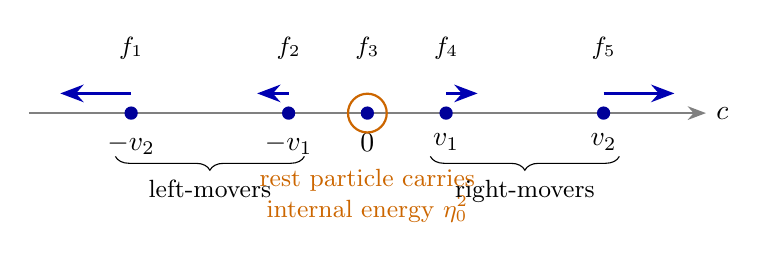
\begin{tikzpicture}[>=Stealth,scale=1.0]
  \draw[->,thick,gray] (-4.3,0) -- (4.3,0) node[right,black] {$c$};
  \foreach \x/\lab/\idx in {-3/{-v_2}/1,-1/{-v_1}/2,0/{0}/3,1/{v_1}/4,3/{v_2}/5}{
    \fill[blue!60!black] (\x,0) circle (2.4pt);
    \node[below=4pt] at (\x,0) {$\lab$};
    \node[above=16pt,font=\small] at (\x,0) {$f_{\idx}$};
  }
  \draw[->,very thick,blue!70!black] (-3,0.25) -- (-3.9,0.25);
  \draw[->,very thick,blue!70!black] (-1,0.25) -- (-1.4,0.25);
  \draw[->,very thick,blue!70!black] (1,0.25) -- (1.4,0.25);
  \draw[->,very thick,blue!70!black] (3,0.25) -- (3.9,0.25);
  \draw[orange!80!black,thick] (0,0) circle (7pt);
  \node[orange!80!black,font=\small,align=center] at (0,-1.05) {rest particle carries\\ internal energy $\eta_0^2$};
  \draw[decorate,decoration={brace,amplitude=5pt,mirror}] (-3.2,-0.55) -- (-0.8,-0.55) node[midway,below=5pt,font=\small] {left-movers};
  \draw[decorate,decoration={brace,amplitude=5pt,mirror}] (0.8,-0.55) -- (3.2,-0.55) node[midway,below=5pt,font=\small] {right-movers};
\end{tikzpicture}
\caption{The KT-D1V5 velocity set.  Arrow lengths are proportional to $|c_i|$.  Only the
rest particle has a nonzero internal-energy coordinate $\eta_3=\eta_0$.}
\label{fig:velset}
\end{figure}

\subsection{Discrete moments and the equilibrium}

The discrete analogues of~\eqref{eq:moments_cont} are
\begin{equation}
  \rho = \sum_{i} f_i,\qquad
  \rho u = \sum_i c_i f_i,\qquad
  2E = \rho(bT+u^2) = \sum_i (c_i^2 + \eta_i^2) f_i .
  \label{eq:moments_disc}
\end{equation}
The equilibrium is required to reproduce, exactly, every moment that appears in the
Euler fluxes: the three conserved densities above, the momentum flux, and the
energy flux,
\begin{gather}
  \sum_i \feq_i = \rho, \qquad
  \sum_i c_i \feq_i = \rho u, \qquad
  \sum_i (c_i^2+\eta_i^2)\feq_i = \rho(bT+u^2), \label{eq:c_cons}\\
  \sum_i c_i^2 \feq_i = p + \rho u^2, \qquad
  \sum_i c_i (c_i^2+\eta_i^2)\feq_i = \rho u\bigl[(b+2)T + u^2\bigr] = 2u(E+p). \label{eq:c_flux}
\end{gather}
Because $c_3 = 0$, the last condition involves only the third moment
$M_3 \equiv \sum_i c_i^3 \feq_i$.  These are five linear conditions on five
unknowns, so the equilibrium is \emph{uniquely determined}.

\begin{proposition}[KT-D1V5 equilibrium]
\label{prop:feq}
Write $F_0 = \feq_3$, $S_k = \feq_{k+} + \feq_{k-}$ and $D_k = \feq_{k+}-\feq_{k-}$ for the
slow ($k=1$, $|c|=v_1$) and fast ($k=2$, $|c|=v_2$) pairs.  The unique solution
of~\eqref{eq:c_cons}--\eqref{eq:c_flux} is
\begin{align}
  F_0 &= \rho\,\frac{(b-1)T}{\eta_0^2}, \label{eq:F0}\\
  S_1 &= \rho\,\frac{v_2^2 - K_2 T - u^2}{v_2^2 - v_1^2}, \qquad
  S_2 = \rho\,\frac{K_1 T + u^2 - v_1^2}{v_2^2 - v_1^2},
  \qquad K_k = \frac{(b-1)v_k^2}{\eta_0^2}+1, \label{eq:S}\\
  D_1 &= \rho u\,\frac{v_2^2 - (b+2)T - u^2}{v_1\,(v_2^2-v_1^2)}, \qquad
  D_2 = \rho u\,\frac{(b+2)T + u^2 - v_1^2}{v_2\,(v_2^2-v_1^2)} . \label{eq:D}
\end{align}
Equivalently $\feq_3 = \rho A_0$ and $\feq_{k\pm} = \rho(A_k \pm B_k v_k u)$ with
\begin{equation}
\begin{aligned}
  A_0 &= \frac{(b-1)T}{\eta_0^2}, &
  A_1 &= \frac{-v_2^2 + K_2T + u^2}{2(v_1^2-v_2^2)}, &
  A_2 &= \frac{-v_1^2 + K_1T + u^2}{2(v_2^2-v_1^2)},\\
  & &
  B_1 &= \frac{-v_2^2 + (b+2)T + u^2}{2v_1^2(v_1^2-v_2^2)}, &
  B_2 &= \frac{-v_1^2 + (b+2)T + u^2}{2v_2^2(v_2^2-v_1^2)},
\end{aligned}
\label{eq:AB}
\end{equation}
which is exactly the form evaluated by the solver.
\end{proposition}

\begin{proof}
The even conditions decouple from the odd ones.  The difference of the energy and
momentum-flux conditions isolates the rest particle,
$\eta_0^2F_0 = \rho(bT+u^2) - \rho(T+u^2)$, that is, $\eta_0^2F_0 = \rho(b-1)T$, giving~\eqref{eq:F0}.
The remaining even conditions $S_1+S_2 = \rho - F_0$ and
$v_1^2S_1 + v_2^2S_2 = \rho(T+u^2)$ form a $2\times2$ system whose solution is~\eqref{eq:S}.
The odd conditions $v_1D_1 + v_2D_2 = \rho u$ and
$v_1^3D_1 + v_2^3D_2 = \rho u[(b+2)T+u^2]$ give~\eqref{eq:D}.  Setting
$S_k = 2\rho A_k$ and $D_k = 2\rho B_k v_k u$ reproduces~\eqref{eq:AB}.
\end{proof}

The equilibrium moments were verified numerically over 2000 random states
$(\rho,u,T)$: all five residuals are below $10^{-14}$.

\subsection{The first unconstrained moment}
\label{sec:M4}
The fourth moment is not constrained, and it is what the model ``chooses'' for the
flux of the energy flux.  From~\eqref{eq:S},
\begin{equation}
  M_4 \equiv \sum_i c_i^4 \feq_i = \rho\bigl(\alpha_0 + \alpha_1 T + \alpha_2 u^2\bigr),\quad
  \alpha_0 = -v_1^2v_2^2,\quad
  \alpha_1 = v_1^2+v_2^2 + \frac{(b-1)v_1^2v_2^2}{\eta_0^2},\quad
  \alpha_2 = v_1^2+v_2^2 .
  \label{eq:M4}
\end{equation}
For the solver's parameters $\alpha_0=-9$, $\alpha_1 = 21.755$ and $\alpha_2 = 10$.
The continuous Maxwellian would instead give
$\int\xi^2(\xi^2+\eta^2)\feq = \rho[u^4 + (b+5)Tu^2 + (b+2)T^2]$, which is quadratic in
$T$ and quartic in $u$.  This mismatch is harmless at the Euler level but controls
the dissipative terms (\cref{sec:ce_discrete}).

\subsection{Negative populations}
\label{sec:negative}
The equilibrium is not a probability distribution.  From~\eqref{eq:S},
the slow pair is negative whenever $T > (v_2^2-u^2)/K_2$ ($T>0.706$ at $u=0$), and
the fast pair becomes negative for $T < (v_1^2-u^2)/K_1$ ($T<0.434$ at $u=0$).
The Sod temperatures lie between $0.711$ and $1.141$, so the slow populations are
negative over almost the entire flow (\cref{fig:feq}).  This is admissible in a
discrete Boltzmann method, where the populations are moment carriers rather than
particle densities, but it has two consequences.  First, no positivity argument
can be made at the population level.  The solver therefore tests only the recovered
$\rho>0$ and $T>0$.  Second, a population-by-population slope limiter
(\cref{sec:limiters}) acts on signed quantities whose extrema have no direct
physical meaning.

\begin{figure}[ht]
\centering
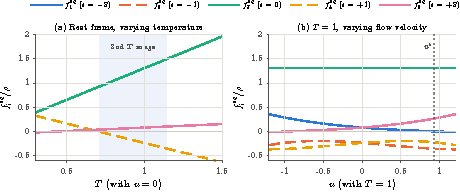
\includegraphics[width=\textwidth]{fig_equilibrium_populations.pdf}
\caption{KT-D1V5 equilibrium populations per unit density.  (a) At $u=0$ the pairs
$f_1=f_5$ and $f_2=f_4$ coincide.  The shaded band is the range of $T$ in the Sod
solution, where the slow populations are negative.  (b) At $T=1$, a nonzero flow
velocity splits each pair.  Near $u^* = 0.927$ the fast population moving against
the flow ($f_1$) approaches zero.}
\label{fig:feq}
\end{figure}

\subsection{Recovering the macroscopic state}
\label{sec:recovery}
The inverse map from populations to primitive variables follows
from~\eqref{eq:moments_disc}:
\begin{equation}
  \rho = \sum_i f_i,\qquad
  u = \frac{1}{\rho}\sum_i c_i f_i,\qquad
  T = \frac1b\left[\frac{1}{\rho}\sum_i (c_i^2+\eta_i^2)f_i - u^2\right],\qquad
  p = \rho T .
  \label{eq:recovery}
\end{equation}
Temperature is the most delicate of these because it is the difference of two
$\ord(1)$ quantities.  Linearizing~\eqref{eq:recovery} gives the sensitivity of $T$ to
a perturbation of one population:
\begin{equation}
  \pd{T}{f_i} = \frac{(c_i-u)^2 + \eta_i^2 - bT}{b\rho}.
  \label{eq:dTdf}
\end{equation}
The weights $\partial T/\partial f_i$ for the Sod states are listed in
\cref{tab:sensitivity}.  In the low-density post-shock state the fast population
travelling against the flow has a weight of about $7.3$.  A reconstruction error in
that single population is amplified about sevenfold in $T$, while density
(weights $\equiv1$) and pressure respond far less.  This is the mechanical reason
why temperature is the first variable to show limiter-induced overshoot
(\cref{sec:limiter_results}).

\begin{table}[ht]
\centering
\caption{Equilibrium populations and temperature sensitivities~\eqref{eq:dTdf} in the
four constant states of the Sod solution.}
\label{tab:sensitivity}
\small
\begin{tabular}{@{}llrrrrr@{}}
\toprule
State $(\rho,u,T)$ & & $i=1$ ($-3$) & $i=2$ ($-1$) & $i=3$ ($0$) & $i=4$ ($+1$) & $i=5$ ($+3$)\\
\midrule
Left $(1,0,1)$ & $\feq_i$ & $0.0816$ & $-0.2347$ & $1.306$ & $-0.2347$ & $0.0816$ \\
 & $\partial T/\partial f_i$ & $0.80$ & $-0.80$ & $-0.39$ & $-0.80$ & $0.80$ \\[2pt]
Right $(0.125,0,0.8)$ & $\feq_i$ & $0.0066$ & $-0.0094$ & $0.1306$ & $-0.0094$ & $0.0066$ \\
 & $\partial T/\partial f_i$ & $8.0$ & $-4.8$ & $-1.5$ & $-4.8$ & $8.0$ \\[2pt]
Star-left $(0.426,0.927,0.711)$ & $\feq_i$ & $0.0001$ & $-0.1029$ & $0.3959$ & $0.0534$ & $0.0798$ \\
 & $\partial T/\partial f_i$ & $5.57$ & $0.08$ & $0.17$ & $-1.67$ & $0.35$ \\[2pt]
Star-right $(0.266,0.927,1.141)$ & $\feq_i$ & $0.0011$ & $-0.1089$ & $0.3959$ & $-0.1042$ & $0.0817$ \\
 & $\partial T/\partial f_i$ & $7.32$ & $-1.50$ & $-1.34$ & $-4.29$ & $-1.06$ \\
\bottomrule
\end{tabular}
\end{table}

% ===========================================================================
\section{Hydrodynamics of the discrete model}
\label{sec:ce_discrete}
% ===========================================================================

The discrete BGK equation solved by the program is, for each population,
\begin{equation}
  \pd{f_i}{t} + c_i\pd{f_i}{x} = \frac{\feq_i(\rho,u,T) - f_i}{\tau},
  \qquad i = 1,\dots,5 .
  \label{eq:dbe}
\end{equation}
Each equation is a linear advection equation with a relaxation source.  The
nonlinearity is confined to $\feq_i$, which depends on all five populations
through~\eqref{eq:recovery}.

\subsection{Exact conservation}
\label{sec:conservation}
Multiplying~\eqref{eq:dbe} by $\psi_i \in \{1,\ c_i,\ \tfrac12(c_i^2+\eta_i^2)\}$ and
summing, the collision term vanishes identically by~\eqref{eq:c_cons}:
$\sum_i\psi_i(\feq_i - f_i) = 0$.  Mass, momentum and energy are therefore
conserved by the collision operator exactly, not approximately, and this property
survives discretization because the equilibrium is rebuilt from the discrete
moments of the current populations.

\subsection{Euler level}
Substituting $f_i=\feq_i$ into the summed equations and using~\eqref{eq:c_flux}
gives~\eqref{eq:euler_mass}--\eqref{eq:euler_energy} exactly.  The five
conditions~\eqref{eq:c_cons}--\eqref{eq:c_flux} are precisely the conditions
needed for this, so the D1V5 model is the minimal discrete velocity model for the
one-dimensional Euler equations with adjustable $\gamma$.

\subsection{First-order Chapman--Enskog analysis}
\label{sec:ce_first}
With $f_i = \feq_i + \tau f_i^{(1)} + \ord(\tau^2)$ and
$f^{(1)}_i = -(\partial_{t_0} + c_i\partial_x)\feq_i$, the $\ord(\tau)$ corrections
to the three fluxes are moments of $f^{(1)}$.  The time derivatives
$\partial_{t_0}$ are replaced by spatial derivatives using the Euler equations in
primitive form,
$\partial_{t_0}\rho = -u\rho_x - \rho u_x$,
$\partial_{t_0}u = -uu_x - p_x/\rho$,
$\partial_{t_0}p = -up_x - \gamma p u_x$.

\paragraph{Mass.}  $\sum_i c_i f_i^{(1)} = -[\partial_{t_0}(\rho u) + \partial_x(p+\rho u^2)] = 0$.
The mass flux has no dissipative correction.

\paragraph{Momentum.}  Using $M_2 = p+\rho u^2$ and $M_3 = \rho u^3 + (b+2)pu$,
\begin{equation}
  \Pi \equiv \tau\sum_i c_i^2 f_i^{(1)} = -\tau\bigl[\partial_{t_0}M_2 + \partial_x M_3\bigr]
  = -\tau(b-1)\bigl(\gamma p\,u_x + u\,p_x\bigr).
  \label{eq:Pi}
\end{equation}
The momentum equation becomes
$\partial_t(\rho u) + \partial_x(\rho u^2 + p) = \partial_x\sigma$ with
$\sigma = -\Pi = \tau(b-1)(\gamma p u_x + u p_x)$.

\paragraph{Energy.}  Using~\eqref{eq:M4}, the energy-flux correction
$\tilde q \equiv \tfrac{\tau}{2}\sum_i c_i(c_i^2+\eta_i^2) f_i^{(1)} = -\tfrac{\tau}{2}[\partial_{t_0}M_3 + \partial_x M_4]$ is
\begin{equation}
  \tilde q = \frac{\tau}{2}\Bigl[P(u)\,\rho_x
   - \bigl(\alpha_1 - (b+2)T - (b+5)u^2\bigr)p_x
   + u\bigl(4\rho u^2 + (b+2)(\gamma+1)p - 2\alpha_2\rho\bigr)u_x\Bigr],
  \label{eq:qtilde}
\end{equation}
where
\begin{equation}
  P(u) \equiv (v_1^2 - u^2)(v_2^2 - u^2) = -\bigl(\alpha_0 + \alpha_2u^2 - u^4\bigr).
  \label{eq:P}
\end{equation}
Both closed forms~\eqref{eq:Pi} and~\eqref{eq:qtilde} were checked against direct
numerical differentiation of the actual equilibrium at 500 random states and
gradients.  The relative discrepancy was below $3\times10^{-9}$ (the finite-difference error).

\subsection{What the discrete model gets right and wrong at $\ord(\tau)$}
\label{sec:ce_compare}

\Cref{tab:ce_compare} compares~\eqref{eq:Pi}--\eqref{eq:qtilde} with the continuous
BGK result~\eqref{eq:bgk_transport}.  Three differences matter.
\begin{enumerate}
  \item \textbf{Viscosity magnitude.}  The coefficient of $u_x$ in the stress is
        $(b-1)\gamma p\tau = 5.6\,p\tau$ instead of $2(1-1/b)p\tau = 1.6\,p\tau$.
  \item \textbf{Galilean invariance.}  The terms $u\,p_x$ in $\sigma$ and the
        explicit $u$-dependence of $\tilde q$ mean that the dissipation depends on
        the velocity of the frame.  A lattice with a finite number of speeds can
        match only finitely many Maxwellian moments.  Galilean invariance of the
        $\ord(\tau)$ terms needs moments beyond those
        in~\eqref{eq:c_cons}--\eqref{eq:c_flux}~\citep{Shan2006}.
  \item \textbf{Spurious density-gradient energy flux.}  At $u=0$,
        $\tilde q = -\tfrac{\tau}{2}\rho(\alpha_1-(b+2)T)\,T_x + \tfrac{\tau}{2}[v_1^2v_2^2 - \alpha_1T + (b+2)T^2]\,\rho_x$.
        The first term is a heat conduction with
        $\kappa_{\mathrm{eff}} = \tfrac{\tau}{2}\rho(\alpha_1 - (b+2)T)$
        ($\approx 7.4\rho\tau$ at $T=1$ versus the BGK value $3.5\rho\tau$).
        The second term is an energy flux driven by density gradients, which has no
        counterpart in the continuous gas.
\end{enumerate}
The conclusion is that, in this model, $\tau$ is not a physical viscosity
parameter.  It is a regularization that vanishes as $\tau\to0$ and leaves the Euler
equations.  The KT D1V5 model is an \emph{Euler} model~\citep{KataokaTsutahara2004Euler};
a Navier--Stokes model requires more velocities~\citep{KataokaTsutahara2004NS}.
This is consistent with using the exact inviscid Sod solution as the reference.

\begin{table}[ht]
\centering
\caption{First-order (in $\tau$) dissipative fluxes: continuous BGK gas versus the
KT-D1V5 model, one-dimensional flow.}
\label{tab:ce_compare}
\small
\renewcommand{\arraystretch}{1.25}
\begin{tabular}{@{}lll@{}}
\toprule
 & Continuous BGK & KT-D1V5 (derived here) \\
\midrule
Mass flux correction & $0$ & $0$ \\
Viscous stress $\sigma$ & $(3-\gamma)\,p\tau\,u_x$ & $(b-1)\tau\,(\gamma p\,u_x + u\,p_x)$ \\
Heat flux at $u=0$ & $-\frac{b+2}{2}p\tau\,T_x$ & $-\frac{\tau}{2}\rho(\alpha_1-(b+2)T)T_x + \frac{\tau}{2}[v_1^2v_2^2-\alpha_1T+(b+2)T^2]\rho_x$ \\
Contact diffusivity $D_c$ & $\tau T$ & $\tau P(U)/[(b+2)T]$ \\
Galilean invariant & yes & no \\
\bottomrule
\end{tabular}
\end{table}

\subsection{Diffusion of a contact discontinuity}
\label{sec:contact_diffusion}

A contact discontinuity moves with the flow velocity $U$ and carries a jump in $\rho$
and $T$ at constant $p$ and $u$.  At a contact $u_x = p_x = 0$ to leading order, so
$\Pi = 0$ and~\eqref{eq:qtilde} reduces to $\tilde q = \tfrac{\tau}{2}P(U)\rho_x$.
Subtracting the kinetic-energy equation from the energy equation gives the
pressure equation
$\tfrac{b}{2}(\partial_t p + up_x) + \tfrac{b+2}{2}pu_x = -\partial_x\tilde q$.
Because pressure equilibrates acoustically much faster than the contact diffuses,
$p$ remains uniform.  The heat flux therefore produces a small dilatation
$u_x = -2\partial_x\tilde q/[(b+2)p]$, and the continuity equation
$D\rho/Dt = -\rho u_x$ becomes a diffusion equation,
\begin{equation}
  \frac{D\rho}{Dt} = D_c\,\rho_{xx},\qquad
  D_c = \frac{\tau\,(v_1^2 - U^2)(v_2^2 - U^2)}{(b+2)\,T}.
  \label{eq:Dc}
\end{equation}
For the continuous BGK gas the same argument gives $D_c = \tau T$.  Two features
of~\eqref{eq:Dc} are notable (\cref{fig:contactD}):
\begin{itemize}
  \item The diffusivity depends on the contact velocity.  At the Sod contact,
        $U = u^* = 0.9275$, the factor $P(U)/P(0) = 0.126$.  The contact therefore
        diffuses about eight times more slowly than it would at rest.
  \item For $v_1 < |U| < v_2$, $D_c<0$.  The discrete model is then
        \emph{anti-diffusive} at contacts, and the $\ord(\tau)$ system is ill-posed.
        The KT-D1V5 model with $v_1 = 1$ can therefore represent a contact only
        if $|U|<v_1$.  The Sod problem, with $u^*/v_1 = 0.93$, sits close to this limit.
\end{itemize}
Starting from a step, the solution of~\eqref{eq:Dc} is an error function of width
$w = \sqrt{4D_ct}$.  Its maximum-gradient thickness, $\delta_c \equiv |[\rho]|/\max|\rho_x|$, is
\begin{equation}
  \delta_c^{\mathrm{kin}} = \sqrt{4\pi D_c t}.
  \label{eq:dkin}
\end{equation}
Using $T\in[T^*_L,T^*_R] = [0.711,1.141]$ and $t = 0.15$ gives
$\delta_c^{\mathrm{kin}} \in [\kinContactMin,\ \kinContactMax]$ for $\tau = 5\times10^{-6}$.
This \emph{kinetic floor} is set by the model, not by the grid.  Even an exact
solution of~\eqref{eq:dbe} would show a contact of this thickness.  An error-function
contact of width $w$ and jump $J$ contributes
\begin{equation}
  \int (\rho-\rho_{\mathrm{Euler}})^2\,\dd x = J^2 w\,\frac{2-\sqrt2}{2\sqrt\pi},
  \label{eq:erf_l2}
\end{equation}
to the squared error.  With $J=\rho^*_L-\rho^*_R = 0.1607$, this sets a floor
of $\rhoFloorMin$--$\rhoFloorMax$ on the global RMS density error defined in
\cref{sec:metrics}.  Grid refinement cannot remove it at fixed $\tau$.

\begin{figure}[ht]
\centering
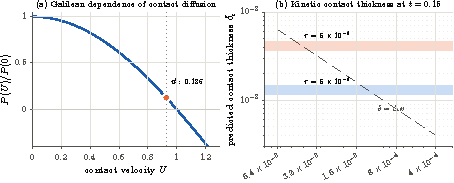
\includegraphics[width=\textwidth]{fig_contact_diffusivity.pdf}
\caption{(a) Velocity dependence of the model's contact diffusivity~\eqref{eq:Dc}.
(b) Predicted kinetic contact thickness~\eqref{eq:dkin} at $t=0.15$ for the present
$\tau$ and for the earlier $\tau=5\times10^{-5}$, compared with the cell size of the
five convergence grids.  The kinetic thickness is less than about four cells even on
the finest grid, so it is only marginally resolved.}
\label{fig:contactD}
\end{figure}

\subsection{Shock thickness and the kinetic resolution parameter}
\label{sec:shock_thickness}
Across the right-moving shock, $u_x$ and $p_x$ are both negative, so the two terms
of $\sigma$ add.  Balancing the stress against the momentum flux through the shock,
$\dot m\,[u] \sim \mu_{\mathrm{eff}}[u]/\delta_s$ with $\dot m = \rho_R S$, gives
\begin{equation}
  \delta_s \sim \frac{\mu_{\mathrm{eff}}}{\rho_R S},\qquad
  \mu_{\mathrm{eff}} \approx (b-1)\tau\Bigl(\gamma\bar p + \bar u\,\frac{[p]}{[u]}\Bigr)\approx 1.5\tau ,
\end{equation}
so $\delta_s \approx 7\tau \approx 3.5\times10^{-5}$.  This is an order of magnitude
smaller than the finest cell ($\Delta x = 4\times10^{-4}$).  The physical shock
structure is therefore never resolved, and the captured shock thickness is set by
the numerical scheme.  A convenient single measure is the \emph{kinetic
resolution parameter}
\begin{equation}
  R_\tau = \frac{\Delta x}{v_2\,\tau},
  \label{eq:Rtau}
\end{equation}
the number of fast-particle relaxation lengths per cell.  It equals $427$, $213$,
$107$, $53$ and $27$ on the five grids.  The solver thus always operates in the
under-resolved-relaxation (hydrodynamic) regime.  The one exception is the
contact, where kinetic diffusion accumulates as $\sqrt{\tau t}$ rather than
scaling with $\tau$ alone.

% ===========================================================================
\section{The Sod shock tube and its exact solution}
\label{sec:sod}
% ===========================================================================

\subsection{Problem statement}
The initial data are two constant states separated by a diaphragm at $x_0=10$:
\begin{equation}
  (\rho,u,p)(x,0) =
  \begin{cases} (1,\ 0,\ 1), & x < x_0,\\ (0.125,\ 0,\ 0.1), & x > x_0. \end{cases}
\end{equation}
The kinetic solver is initialized at local equilibrium, $f_i(x,0) = \feq_i(\rho,u,T)$,
so no initial non-equilibrium layer is imposed.

\subsection{Exact Riemann solution}
\label{sec:riemann}
The Euler Riemann problem is self-similar in $\xi = (x-x_0)/t$ and consists of a
left wave, a contact discontinuity moving at $u^*$, and a right wave, separating
two ``star'' states with common $p^*$ and $u^*$~\citep{Toro2009}.  The star pressure
is the root of
\begin{equation}
  \mathcal F(p) \equiv f_L(p) + f_R(p) + (u_R - u_L) = 0,
  \label{eq:pressure_function}
\end{equation}
where, for $K\in\{L,R\}$,
\begin{equation}
  f_K(p) =
  \begin{cases}
    (p-p_K)\left[\dfrac{A_K}{p + B_K}\right]^{1/2}, & p > p_K\ \text{(shock)},\\[10pt]
    \dfrac{2a_K}{\gamma-1}\left[\left(\dfrac{p}{p_K}\right)^{\frac{\gamma-1}{2\gamma}} - 1\right], & p \le p_K\ \text{(rarefaction)},
  \end{cases}
\end{equation}
with $A_K = 2/[(\gamma+1)\rho_K]$ and $B_K = p_K(\gamma-1)/(\gamma+1)$.
The shock branch follows from the Rankine--Hugoniot conditions
$[\rho(u-S)] = 0$, $[\rho u(u-S) + p] = 0$, $[E(u-S) + pu] = 0$.  The rarefaction
branch follows from constancy of the Riemann invariant $u + 2a/(\gamma-1)$ and of
entropy $p/\rho^\gamma$ through the fan.  $\mathcal F$ is monotone and concave, so
Newton's method,
$p^{(k+1)} = p^{(k)} - \mathcal F(p^{(k)})/\mathcal F'(p^{(k)})$, converges from
$p^{(0)} = \tfrac12(p_L+p_R)$.  Then $u^* = \tfrac12(u_L+u_R) + \tfrac12[f_R(p^*) - f_L(p^*)]$.

For Sod, $p^* < p_L$ (left rarefaction) and $p^* > p_R$ (right shock).  Inside the fan,
$\xi\in[u_L-a_L,\ u^*-a^*_L]$,
\begin{equation}
  u = \frac{2}{\gamma+1}\Bigl(a_L + \xi\Bigr),\quad
  a = \frac{2}{\gamma+1}\Bigl(a_L - \tfrac{\gamma-1}{2}\xi\Bigr),\quad
  \rho = \rho_L\Bigl(\frac{a}{a_L}\Bigr)^{\frac{2}{\gamma-1}},\quad
  p = p_L\Bigl(\frac{a}{a_L}\Bigr)^{\frac{2\gamma}{\gamma-1}} .
\end{equation}
Behind the shock, $\rho^*_R = \rho_R\,\dfrac{p^*/p_R + \frac{\gamma-1}{\gamma+1}}{\frac{\gamma-1}{\gamma+1}p^*/p_R + 1}$,
and the shock speed is $S = a_R\sqrt{\frac{\gamma+1}{2\gamma}\frac{p^*}{p_R} + \frac{\gamma-1}{2\gamma}}$.
The resulting constants (\cref{tab:sod}, \cref{fig:exact}) are used throughout.

\begin{table}[ht]
\centering
\caption{Exact Sod constants ($\gamma = 1.4$) and wave positions at $t=0.15$.}
\label{tab:sod}
\small
\begin{tabular}{@{}llll@{}}
\toprule
Quantity & Value & Wave & Speed $\to$ position $x-x_0$ \\
\midrule
$p^*$ & $0.303130$ & rarefaction head & $-1.18322 \to -0.17748$ \\
$u^*$ & $0.927453$ & rarefaction tail & $-0.07027 \to -0.01054$ \\
$\rho^*_L,\ T^*_L$ & $0.426319,\ 0.711040$ & contact & $\phantom{-}0.92745 \to \phantom{-}0.13912$ \\
$\rho^*_R,\ T^*_R$ & $0.265574,\ 1.141416$ & shock & $\phantom{-}1.75216 \to \phantom{-}0.26282$ \\
Shock Mach number & $1.6556$ & & \\
\bottomrule
\end{tabular}
\end{table}

\begin{figure}[ht]
\centering
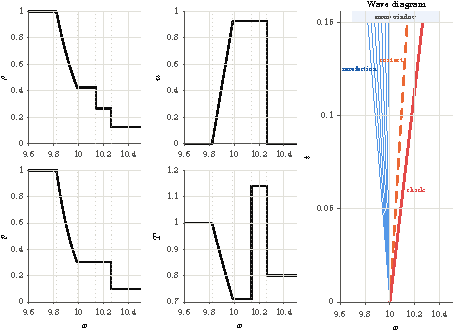
\includegraphics[width=\textwidth]{fig_exact_sod.pdf}
\caption{Exact Euler solution at $t=0.15$ (left, dotted lines mark the four wave
positions) and the $x$--$t$ wave diagram (right).  The shaded strip is the fixed
error window $x_0-0.30\le x\le x_0+0.40$ used for the wave-region metrics.}
\label{fig:exact}
\end{figure}

\paragraph{Why the kinetic solution differs from the Euler reference.}
The DBM solution converges to this inviscid solution only in the double limit
$\Delta x\to0$ and $\tau\to0$.  At fixed $\tau$ and $\Delta x\to0$, it converges
instead to the solution of~\eqref{eq:dbe}.  That solution has a smooth contact of
thickness~\eqref{eq:dkin}, a shock of thickness $\ord(\tau)$, and rounded
rarefaction corners.  The measured error therefore always contains a model
component in addition to the discretization error.

% ===========================================================================
\section{Finite-volume discretization of the transport term}
\label{sec:fv}
% ===========================================================================

\subsection{Cell averages and the semi-discrete equation}
The domain $[0,L_x]$ is divided into $N_x$ cells
$I_j = [x_{j-1/2},x_{j+1/2}]$ of width $\Delta x = L_x/N_x$ with centres
$x_j = (j-\tfrac12)\Delta x$.  Integrating~\eqref{eq:dbe} over $I_j$ and dividing by
$\Delta x$ gives the exact relation
\begin{equation}
  \frac{\dd \bar f_{i,j}}{\dd t} = -\frac{F_{i,j+1/2} - F_{i,j-1/2}}{\Delta x}
     + \frac{\overline{\feq_i}_{\,j} - \bar f_{i,j}}{\tau},
  \qquad F_{i,j+1/2} = c_i\,f_i(x_{j+1/2},t),
  \label{eq:semidiscrete}
\end{equation}
where overbars denote cell averages.  The scheme approximates the cell-averaged
equilibrium by the equilibrium of the cell averages, $\feq_i(\bar\rho_j,\bar u_j,\bar T_j)$.
This is a second-order approximation in smooth flow.  Writing the right-hand side
of~\eqref{eq:semidiscrete} as $\mathcal L(\bar{\mathbf f})$ gives the
method-of-lines system $\dd\bar{\mathbf f}/\dd t = \mathcal L(\bar{\mathbf f})$
that is integrated in time in \cref{sec:time}.

Because the flux enters as a difference of face values, summing over cells
telescopes.  The total amount of any population, and hence of mass, momentum and
energy, changes only through the boundary faces.  The finite-volume scheme is
conservative by construction.

\subsection{Upwind flux: the exact Riemann solver for each population}
Each population obeys a linear advection equation with constant speed $c_i$.  The
Riemann problem at a face with left and right states $f^-$ and $f^+$ has the exact
solution ``take the upstream value''.  The Godunov flux is therefore the upwind flux
\begin{equation}
  F_{i,j+1/2} = c_i^+ f^-_{i,j+1/2} + c_i^- f^+_{i,j+1/2},\qquad
  c^\pm = \tfrac12\bigl(c\pm|c|\bigr),
  \label{eq:upwind}
\end{equation}
and $F=0$ for the rest particle.  Summed over populations, \eqref{eq:upwind}
splits the macroscopic flux into contributions from right-movers and left-movers.
This is the discrete-velocity analogue of kinetic flux-vector
splitting~\citep{MandalDeshpande1994}.  Upwinding happens separately for each
population and needs no characteristic decomposition of the Euler system.  The
kinetic model provides the wave decomposition automatically.

\subsection{Modified equation: numerical diffusion}
\label{sec:modified}
If $f^\pm$ are the cell averages (first-order upwind), a Taylor expansion of the
semi-discrete scheme gives the modified equation~\citep{WarmingHyett1974}
\begin{equation}
  \pd{f_i}{t} + c_i\pd{f_i}{x} = \frac{|c_i|\Delta x}{2}\pd{^2 f_i}{x^2}
    - \frac{c_i\Delta x^2}{6}\pd{^3 f_i}{x^3} + \cdots + \frac{\feq_i - f_i}{\tau}.
\end{equation}
Taking moments with $f_i\approx\feq_i$ shows how the population-level numerical
diffusion reaches the macroscopic equations.  For example, the continuity equation
gains the numerical flux
\begin{equation}
  F_\rho^{\mathrm{num}} = -\frac{\Delta x}{2}\partial_x\sum_i|c_i|\feq_i
  = -\frac{\Delta x}{2}\partial_x\bigl(v_1S_1 + v_2S_2\bigr) \neq 0 .
\end{equation}
First-order kinetic upwinding therefore diffuses mass, momentum and energy with an
effective coefficient of order $v_2\Delta x/2$.  Comparing this with the model
dissipation of order $\tau\cdot\ord(1)$ reproduces the resolution
parameter~\eqref{eq:Rtau}: numerical dissipation dominates whenever $R_\tau\gg1$.
This is why a second-order reconstruction is essential.

\subsection{MUSCL reconstruction}
MUSCL~\citep{vanLeer1979} replaces the piecewise-constant data by a piecewise-linear
reconstruction inside each cell,
\begin{equation}
  f_i(x) \approx \bar f_{i,j} + \sigma_{i,j}\,\frac{x - x_j}{\Delta x},\qquad x\in I_j,
\end{equation}
so the two face states are
\begin{equation}
  f^-_{i,j+1/2} = \bar f_{i,j} + \tfrac12\sigma_{i,j},\qquad
  f^+_{i,j+1/2} = \bar f_{i,j+1} - \tfrac12\sigma_{i,j+1}.
  \label{eq:muscl_faces}
\end{equation}
With the unlimited central slope $\sigma_j = \tfrac12(\bar f_{j+1} - \bar f_{j-1})$, the
$\ord(\Delta x)$ diffusion term cancels, and the leading truncation error becomes the
dispersive term $\ord(\Delta x^2)\,\partial_x^3 f$ (Fromm's scheme).  Unlimited
reconstruction creates new extrema at discontinuities (Godunov's
theorem~\citep{LeVeque2002}), so the slope is limited.

\begin{figure}[ht]
\centering
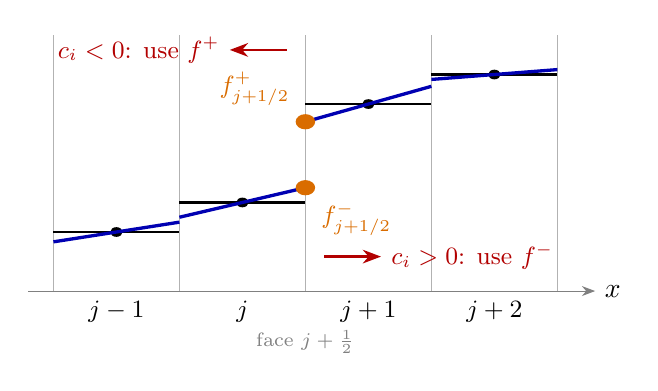
\begin{tikzpicture}[>=Stealth,xscale=1.6,yscale=1.25]
  \foreach \i in {0,...,4}{ \draw[gray!60] (\i,0) -- (\i,2.6); }
  \draw[->,gray] (-0.2,0) -- (4.3,0) node[right,black] {$x$};
  \node[below,font=\small] at (0.5,0) {$j-1$};
  \node[below,font=\small] at (1.5,0) {$j$};
  \node[below,font=\small] at (2.5,0) {$j+1$};
  \node[below,font=\small] at (3.5,0) {$j+2$};
  \node[below,font=\scriptsize,gray] at (2,-0.3) {face $j+\tfrac12$};
  % cell averages
  \foreach \x/\y in {0.5/0.6,1.5/0.9,2.5/1.9,3.5/2.2}{
    \draw[thick,black] (\x-0.5,\y) -- (\x+0.5,\y);
    \fill (\x,\y) circle (1.4pt);
  }
  % limited slopes
  \draw[very thick,blue!70!black] (1,0.75) -- (2,1.05);
  \draw[very thick,blue!70!black] (2,1.72) -- (3,2.08);
  \draw[very thick,blue!70!black] (0,0.5) -- (1,0.7);
  \draw[very thick,blue!70!black] (3,2.15) -- (4,2.25);
  \fill[orange!85!black] (2,1.05) circle (2.2pt);
  \node[orange!85!black,font=\small,anchor=north west] at (2.05,1.0) {$f^-_{j+1/2}$};
  \fill[orange!85!black] (2,1.72) circle (2.2pt);
  \node[orange!85!black,font=\small,anchor=south east] at (1.95,1.78) {$f^+_{j+1/2}$};
  \draw[->,thick,red!70!black] (2.15,0.35) -- (2.6,0.35) node[right,font=\small] {$c_i>0$: use $f^-$};
  \draw[->,thick,red!70!black] (1.85,2.45) -- (1.4,2.45) node[left,font=\small] {$c_i<0$: use $f^+$};
\end{tikzpicture}
\caption{MUSCL reconstruction and upwind face selection for one population.
Black: cell averages; blue: limited linear reconstructions; orange: the two face
states at $x_{j+1/2}$.  The sign of $c_i$ selects which state enters the flux.}
\label{fig:muscl}
\end{figure}

\subsection{Slope limiters}
\label{sec:limiters}

Let $\Delta_{j-1/2} = \bar f_j - \bar f_{j-1}$ and $\Delta_{j+1/2} = \bar f_{j+1} - \bar f_j$.
With
\[
  \minmod(a_1,\dots,a_m) =
  \begin{cases}
  \min_k a_k & \text{if all } a_k>0,\\
  \max_k a_k & \text{if all } a_k<0,\\
  0 & \text{otherwise},
  \end{cases}
\]
the three limiters used in the project are
\begin{align}
  \text{minmod:}&\quad \sigma_j = \minmod(\Delta_{j-1/2},\ \Delta_{j+1/2}),\\
  \text{MC~\citep{vanLeer1977}:}&\quad \sigma_j = \minmod\bigl(2\Delta_{j-1/2},\ \tfrac12(\Delta_{j-1/2}+\Delta_{j+1/2}),\ 2\Delta_{j+1/2}\bigr),\\
  \text{generalized minmod~\citep{KurganovTadmor2000}:}&\quad
  \sigma_j = \minmod\bigl(\theta\Delta_{j-1/2},\ \tfrac12(\Delta_{j-1/2}+\Delta_{j+1/2}),\ \theta\Delta_{j+1/2}\bigr),\quad 1\le\theta\le2 .
  \label{eq:gminmod}
\end{align}
The generalized family contains the other two.  At $\theta=2$ it is MC.  At
$\theta=1$ the centred candidate always lies between the two one-sided candidates,
so it is never the minimum in magnitude, and the family reduces to minmod.  The
solver uses $\theta = 1.2$.

\paragraph{Sweby form.}  Dividing by $\Delta_{j+1/2}$ and writing
$r_j = \Delta_{j-1/2}/\Delta_{j+1/2}$ gives $\sigma_j = \phi(r_j)\Delta_{j+1/2}$ with
\begin{equation}
  \phi_\theta(r) = \max\Bigl[0,\ \min\Bigl(\theta r,\ \tfrac{1+r}{2},\ \theta\Bigr)\Bigr].
  \label{eq:phi}
\end{equation}
For $r\le0$ (a local extremum), $\phi=0$ and the scheme is first order locally.
For $r>0$ the selected candidate changes at $r = 1/(2\theta-1)$ and
$r = 2\theta-1$.  For $\theta = 1.2$ the left candidate is active for $r<0.714$,
the centred candidate for $0.714<r<1.4$, and the right candidate beyond that
(\cref{fig:sweby}b).  Thus $\theta = 1.2$ differs from minmod only in the window
$0.714<r<1.4$ and in the caps $\theta r$ and $\theta$, which allow slopes up to
$20\%$ steeper than a one-sided difference.  Every member satisfies $\phi(1)=1$, so
the reconstruction is exact for linear data and second order in smooth monotone
regions.  Each member also satisfies the symmetry $\phi(r)/r = \phi(1/r)$, so
increasing and decreasing data are treated alike.

\begin{proposition}[TVD range of $\theta$]
\label{prop:tvd}
For a single population with $c>0$, apply the reconstruction~\eqref{eq:muscl_faces}
with the limiter~\eqref{eq:phi} and advance with forward Euler, using
$\nu = c\Delta t/\Delta x$.  The scheme is total-variation diminishing if
$1\le\theta\le2$ and $\nu\le 2/(2+\theta)$.
\end{proposition}
\begin{proof}
The update can be written $\bar f^{n+1}_j = \bar f_j - C_{j-1/2}\Delta_{j-1/2}$ with
$C_{j-1/2} = \nu\bigl[1 + \tfrac12\phi(r_j)/r_j - \tfrac12\phi(r_{j-1})\bigr]$.
By Harten's lemma~\citep{Harten1983}, the scheme is TVD if $0\le C_{j-1/2}\le1$.
From~\eqref{eq:phi}, $0\le\phi(r)\le\theta$ and $0\le\phi(r)/r\le\theta$.  Hence
$\nu(1-\theta/2)\le C\le\nu(1+\theta/2)$.  The lower bound is non-negative only if
$\theta\le2$, and the upper bound is at most one if $\nu\le 2/(2+\theta)$.  The
condition $\theta\ge1$ keeps $\phi$ inside the second-order region
of~\citet{Sweby1984}.
\end{proof}

This shows why $\theta$ is restricted to $[1,2]$: $\theta>2$ breaks the TVD
property.  For $\theta=1.2$ the per-population TVD limit is $\nu\le0.625$.  The
solver's largest population Courant number is $\nu_{\max} = v_2\Delta t/\Delta x \le 0.0094$,
nearly seventy times smaller.  Two caveats apply:
\begin{itemize}
  \item TVD holds for each population's \emph{transport}.  The collision term couples
        the populations through $\feq(\rho,u,T)$, so TVD of the full system, or
        monotonicity of $\rho$, $u$, $p$ or $T$, is not guaranteed.
  \item Limiting is population by population, while $T$ is the nonlinear
        combination~\eqref{eq:recovery}.  A slope that is admissible for every
        $f_i$ separately can still create an extremum in $T$.  This happens most
        easily through the high-sensitivity populations of \cref{tab:sensitivity}.
\end{itemize}

\begin{figure}[ht]
\centering
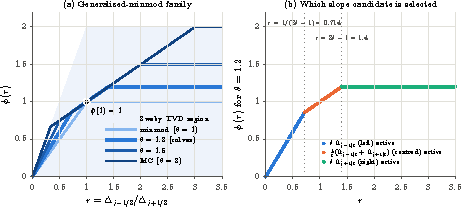
\includegraphics[width=\textwidth]{fig_sweby_diagram.pdf}
\caption{(a) Generalized-minmod limiter functions~\eqref{eq:phi} inside Sweby's TVD
region $0\le\phi\le\min(2r,2)$.  All members pass through $\phi(1)=1$.
(b) For $\theta=1.2$, which of the three candidate slopes is selected, as a
function of the smoothness ratio $r$.}
\label{fig:sweby}
\end{figure}

\paragraph{History of the limiter choice.}  In the project, minmod proved robust but
diffusive, and MC proved sharper but produced a temperature overshoot.  Two binary
hybrids were also tried: one switched per population, and one switched on a shared
macroscopic troubled-cell mask.  The per-population switch was inconsistent with
moment recovery, and the shared mask was threshold-sensitive.  The generalized
minmod replaces the switch with a single continuous parameter, and its
consequences are quantified in \cref{sec:limiter_results}.

\subsection{Boundary treatment}
The first and last cells copy their interior neighbours after every stage, and the
boundary face fluxes copy the adjacent interior face flux.  This zero-gradient
condition is exact while the domain ends remain in their undisturbed states.  At
$t=0.15$ the rarefaction head and the shock are more than $9.7$ units from the
boundaries, so boundary effects are absent (\cref{sec:conservation_results}).

% ===========================================================================
\section{Time integration}
\label{sec:time}
% ===========================================================================

\subsection{SSP-RK3}
The semi-discrete system $\dd\mathbf f/\dd t = \mathcal L(\mathbf f)$, with
$\mathcal L$ = transport + collision, is advanced by the three-stage, third-order
strong-stability-preserving Runge--Kutta method of Shu and
Osher~\citep{ShuOsher1988,Gottlieb2001}:
\begin{align}
  \mathbf f^{(1)} &= \mathbf f^n + \Delta t\,\mathcal L(\mathbf f^n), \nonumber\\
  \mathbf f^{(2)} &= \tfrac34\mathbf f^n + \tfrac14\bigl[\mathbf f^{(1)} + \Delta t\,\mathcal L(\mathbf f^{(1)})\bigr], \label{eq:ssprk3}\\
  \mathbf f^{n+1} &= \tfrac13\mathbf f^n + \tfrac23\bigl[\mathbf f^{(2)} + \Delta t\,\mathcal L(\mathbf f^{(2)})\bigr]. \nonumber
\end{align}
Each stage is a convex combination of forward-Euler steps.  Therefore any convex
functional that is non-increasing under forward Euler, such as total variation or a
maximum norm, remains non-increasing under~\eqref{eq:ssprk3} with the same
time-step restriction (SSP coefficient $1$).  The equivalent Butcher tableau has
nodes $(0,1,\tfrac12)$ and weights $(\tfrac16,\tfrac16,\tfrac23)$.

\subsection{Linear stability}
For $\dd y/\dd t = \lambda y$, one step multiplies $y$ by
\begin{equation}
  R(z) = 1 + z + \frac{z^2}{2} + \frac{z^3}{6},\qquad z = \lambda\Delta t ,
\end{equation}
which matches $e^z$ to third order.  The stability region $|R(z)|\le1$
(\cref{fig:rk3}) contains the real interval $[-2.513,0]$ and the imaginary
interval $|{\rm Im}\,z|\le\sqrt3$.

\paragraph{Collision stiffness.}  Linearize the collision term about any state.
Its Jacobian is $\tau^{-1}(\partial\feq/\partial\mathbf f - I)$.  Because $\feq$
depends on $\mathbf f$ only through the three conserved moments and reproduces
them exactly, $\partial\feq/\partial\mathbf f$ is a projection with eigenvalues
$\{1,1,1,0,0\}$ (confirmed numerically).  The collision spectrum is therefore
exactly $\{0,0,0,-\tau^{-1},-\tau^{-1}\}$: the conserved moments do not relax, and
the two non-conserved modes relax at rate $1/\tau$.  Explicit stability requires
$\Delta t\le 2.513\tau$.  The solver uses
$\Delta t_{\mathrm{col}} = \tau/4$ ($z=-0.25$), for which
$R(-0.25) = 0.778646$ versus $e^{-0.25} = 0.778801$.  This is a relative decay
error of $2\times10^{-4}$ per step, so the relaxation is resolved accurately, not
merely stably.  The forward-Euler collision step
$f + \tfrac{\Delta t}{\tau}(\feq-f)$ is a convex combination of $f$ and $\feq$ for
$\Delta t\le\tau$.

\paragraph{Transport spectrum.}  With the unlimited MUSCL slope, the Fourier symbol of
the semi-discrete transport operator for a population with $c>0$ is
$\lambda(k)\Delta t = -\nu(1-e^{-ik})\bigl(1 + \tfrac{i}{2}\sin k\bigr)$.
For the finest grid ($\nu = 0.0094$) this curve lies deep inside the stability region
(\cref{fig:rk3}b).

\begin{figure}[ht]
\centering
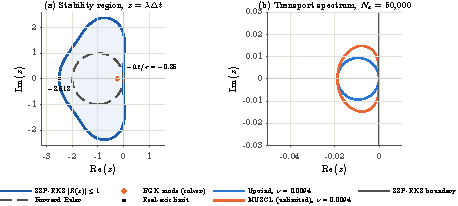
\includegraphics[width=\textwidth]{fig_rk3_stability.pdf}
\caption{(a) SSP-RK3 absolute-stability region with the solver's BGK eigenvalue
$z=-\Delta t/\tau=-0.25$.  (b) Transport spectra for upwind and unlimited MUSCL
reconstruction at the finest grid's Courant number, near the origin.}
\label{fig:rk3}
\end{figure}

\subsection{Time-step selection}
\label{sec:dt}
The solver takes
\begin{equation}
  \Delta t = \min\Bigl(\underbrace{\mathrm{CFL}\,\frac{\Delta x}{v_2}}_{\Delta t_{\mathrm{adv}}},\ \underbrace{\tfrac14\tau}_{\Delta t_{\mathrm{col}}}\Bigr),
  \qquad \nu_{\mathrm{eff}} = \frac{v_2\Delta t}{\Delta x}.
  \label{eq:dt}
\end{equation}
With $\tau=5\times10^{-6}$, $\Delta t_{\mathrm{col}}=1.25\times10^{-6}$.  With
$\mathrm{CFL}=0.025$, $\Delta t_{\mathrm{adv}}$ ranges from $5.3\times10^{-5}$ ($N_x=3125$)
down to $3.3\times10^{-6}$ ($N_x=50{,}000$).  The collision limit therefore controls
on \emph{every} grid.  All five runs use the same $\Delta t=1.25\times10^{-6}$ and
the same number of steps.  The effective Courant number $\nu_{\mathrm{eff}}$ doubles
with each refinement, from $5.9\times10^{-4}$ to $9.4\times10^{-3}$, while the CFL
input never becomes active.  Two consequences follow:
\begin{enumerate}
  \item The convergence study is a pure spatial refinement at fixed $\Delta t$.  It
        is not a refinement at constant Courant number.
  \item Because $\nu_{\mathrm{eff}}\le 0.0094$ and $\Delta t/\tau = 0.25$, temporal error
        is expected to be far below spatial error.  No separate time-step
        refinement was run for this report, so this is an expectation rather than a
        measurement.
\end{enumerate}

\subsection{Stage checks and fallback}
After every stage the solver recovers $(\rho,T)$ and rejects the step if either is
non-positive or non-finite.  A rejected step is retried with $\Delta t/2$.  From the
fifth retry onward it uses minmod, and from the ninth first-order upwind.  Positivity
repair (clipping) is disabled.  All runs reported here completed with zero retries
and zero fallbacks, so every result is a pure generalized-minmod solution.

\begin{algorithm}[ht]
\caption{One accepted time step of the solver}
\label{alg:step}
\begin{algorithmic}[1]
\Function{RHS}{$\mathbf f$}
  \State $(\rho,u,T)\gets$ moments of $\mathbf f$ by~\eqref{eq:recovery}
  \State $\feq\gets$ KT-D1V5 equilibrium~\eqref{eq:AB}
  \For{each population $i$}
     \State limited slopes $\sigma_{i,j}$ by~\eqref{eq:gminmod}; face states by~\eqref{eq:muscl_faces}
     \State upwind face fluxes by~\eqref{eq:upwind}; divergence $(F_{j+1/2}-F_{j-1/2})/\Delta x$
  \EndFor
  \State \Return $-\text{divergence} + (\feq - \mathbf f)/\tau$
\EndFunction
\State $\Delta t\gets$~\eqref{eq:dt}
\Repeat
  \State three SSP-RK3 stages~\eqref{eq:ssprk3}, zero-gradient boundaries after each
  \State \textbf{if} any stage has $\rho\le0$ or $T\le0$: $\Delta t\gets\Delta t/2$, retry (fallback limiters after 4 and 8 retries)
\Until{all stages physical}
\end{algorithmic}
\end{algorithm}

% ===========================================================================
\section{Error measures and what to expect from them}
\label{sec:metrics}
% ===========================================================================

\subsection{Definitions}
For a field $q$ with numerical cell values $q_j$ and exact values $q^{\mathrm{ex}}_j$
evaluated at the cell centres, the solver reports
\begin{align}
  L_1(q) &= \frac1{N}\sum_{j}|q_j - q^{\mathrm{ex}}_j|, &
  L_2(q) &= \Bigl[\frac1{N}\sum_{j}(q_j - q^{\mathrm{ex}}_j)^2\Bigr]^{1/2}, \label{eq:norms}
\end{align}
over all $N=N_x$ cells (global) or over the $N_W$ cells in the fixed window
$W = [x_0-0.30,\ x_0+0.40]$ (wave region).  These are mean and root-mean-square
errors.  Since $N\Delta x = L_x$ is fixed, they equal $L_x^{-1}\|e\|_{L^1}$ and
$L_x^{-1/2}\|e\|_{L^2}$, so observed orders are unaffected by the normalization.
Because the undisturbed part of the domain is $19.56/20$ of its length, global
values are diluted by a factor of about $W/L_x = 0.035$ ($L_1$) or $\sqrt{0.035}$ ($L_2$)
relative to wave-region values.
The temperature peak excess
$\max_{W}T - \max_{W}T^{\mathrm{ex}}$ measures overshoot above the exact post-shock
value $T^*_R=1.1414$.

The observed order between two grids and the least-squares order over all grids are
\begin{equation}
  p_{k} = \frac{\ln(E_{k-1}/E_{k})}{\ln(\Delta x_{k-1}/\Delta x_{k})},\qquad
  \ln E = \ln C + p\ln\Delta x\ \ \text{(fit)} ,
  \label{eq:order}
\end{equation}
following standard verification practice~\citep{Roache1998,OberkampfRoy2010}.

\subsection{Expected rates for discontinuous solutions}
\label{sec:expected_rates}
The Sod solution is not smooth, so the formal second-order accuracy of MUSCL does not
translate into second-order convergence of these norms.  Suppose a
discontinuity with jump $J$ is smeared over a thickness $\delta$.  The error is
$\ord(J)$ over a length $\ord(\delta)$, so
\begin{equation}
  L_1 \propto J\,\delta,\qquad L_2\propto J\,\delta^{1/2} .
  \label{eq:L1L2delta}
\end{equation}
The $L_2$ rate is therefore half the $L_1$ rate.  How $\delta$ scales with $\Delta x$
depends on the wave:
\begin{itemize}
\item \textbf{Shock.}  Characteristics converge into a shock, which balances numerical
      diffusion and keeps $\delta_s = \ord(\Delta x)$ (a fixed number of cells).  Hence
      $L_1\propto\Delta x$ and $L_2\propto\Delta x^{1/2}$.
\item \textbf{Contact.}  A contact is linearly degenerate, so nothing counteracts
      numerical diffusion and it keeps spreading.  For a method of order $m$ the
      smeared width grows like $\delta_c\propto(\Delta x^{m}t)^{1/(m+1)}$
      \citep{Harten1977,LeVeque2002}.  That gives $\delta_c\propto\Delta x^{1/2}$
      for first order and $\Delta x^{2/3}$ for second order.  The corresponding
      rates are $L_1\propto\Delta x^{2/3}$ and $L_2\propto\Delta x^{1/3}$ for MUSCL.
      The classical results on discontinuous data~\citep{Kuznetsov1976,BrennerThomeeWahlbin1975}
      bound these rates from below.
\item \textbf{Rarefaction.}  The rarefaction is continuous with kinks at its head and
      tail, so its error converges faster than either discontinuity.
\end{itemize}
Since the global squared error is the sum of the squared contributions of the
three waves, the asymptotic $L_2$ rate is the \emph{slowest} of the three, which is
$1/3$ from the contact.  At fixed $\tau$ there is also the model floor of
\cref{sec:contact_diffusion}.  Once $\delta_c^{\mathrm{num}}\lesssim\delta_c^{\mathrm{kin}}$,
the contact error stops decreasing.  Heuristically,
\begin{equation}
  E_{L_2}^2 \approx C_s\,\Delta x + C_c\bigl[(\delta_c^{\mathrm{num}})^2 + (\delta_c^{\mathrm{kin}})^2\bigr]^{1/2} + E_{\mathrm{raref}}^2 .
  \label{eq:error_model}
\end{equation}
Observed global $L_2$ orders between about $1/3$ and $1/2$ are therefore the
\emph{correct} behaviour for a second-order shock-capturing method on this problem.
They are not a symptom of a defect.

% ===========================================================================
\section{Results}
\label{sec:results}
% ===========================================================================

% ---------------------------------------------------------------------------
% Results.  Every table body below is written by make_results_figures.m.
% ---------------------------------------------------------------------------

All runs use the configuration of \cref{tab:config}.  The convergence study was
executed with \file{run_d1v5_gminmod_L2_convergence.m}.  The limiter comparison
and the $\theta$-sweep use $N_x = 6250$ with the same $\tau$, CFL and final time.

\subsection{Run summary and conservation}
\label{sec:conservation_results}

\Cref{tab:runs} confirms the time-step analysis of \cref{sec:dt}.  Every grid used
$\Delta t = \tau/4$, the same $120{,}001$ steps (the last is a round-off-sized remainder that lands
exactly on $t_{\mathrm{end}}$), and no retries or fallbacks.  \Cref{tab:conservation} checks the
conservation argument of \cref{sec:conservation}.  Mass and energy are conserved to
round-off relative to the discrete initial condition.  The momentum equals
$(p_L-p_R)\,t_{\mathrm{end}} = 0.135$ to round-off, because the undisturbed boundary
states exert the net pressure force $p_L - p_R$ on the domain.

\begin{table}[ht]
\centering
\caption{Convergence runs: grid spacing, time step, effective Courant number
$\nu_{\mathrm{eff}} = v_2\Delta t/\Delta x$, number of steps, and stability events.}
\label{tab:runs}
\small
\begin{tabular}{@{}rccccrr@{}}
\toprule
$N_x$ & $\Delta x$ & $\Delta t$ & $\nu_{\mathrm{eff}}$ & steps & retries & fallbacks \\
\midrule
\tabinput{data/tab_conv_setup.tex}
\bottomrule
\end{tabular}
\end{table}

\begin{table}[ht]
\centering
\caption{Conservation errors at $t=0.15$: $\sum_j q_j\Delta x$ minus its expected value
(mass and energy: discrete initial value; momentum: $(p_L-p_R)t$).}
\label{tab:conservation}
\small
\begin{tabular}{@{}rccc@{}}
\toprule
$N_x$ & mass & momentum & energy \\
\midrule
\tabinput{data/tab_conservation.tex}
\bottomrule
\end{tabular}
\end{table}

\paragraph{Odd grid.}  $N_x=3125$ is odd, so the cell centre $x_{1563}$ coincides with
the diaphragm.  The solver assigns cells with $x_j<x_0$ to the left state, so that
cell receives the right state.  The discrete diaphragm therefore sits at
$x_0-\Delta x/2$.  This is an $\ord(\Delta x)$ initial-condition offset present only
on the coarsest grid.  It contributes to that grid's contact position error
(\cref{tab:features}) and to the first pairwise orders.

\subsection{The computed solution}

\Cref{fig:finest} compares the $N_x = 50{,}000$ solution with the exact Euler
solution, and \cref{fig:gridzoom} shows how each wave sharpens under refinement.
The profiles are free of oscillations, and the four constant states are reproduced
to plotting accuracy.  The pointwise error is concentrated in a few cells at each
wave.  The largest errors occur at the shock in every variable and at the contact
in $\rho$ and $T$.  The rarefaction head and tail show small corner errors.  The
largest of these is a slight density undershoot just behind the tail
(\cref{fig:gridzoom}a), which is limited in amplitude and shrinks with $\Delta x$.
The maximum pointwise error does not decrease with $\Delta x$: it stays at
$\approx0.08$ in $\rho$ and $0.34$--$0.63$ in $u$.  This is expected, because an
$\ord(1)$ jump spread over a few cells always leaves an $\ord(1)$ error in the cell
that straddles it.

\begin{figure}[p]
\centering
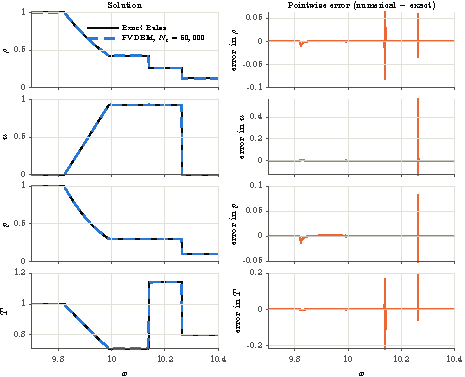
\includegraphics[width=\textwidth]{fig_solution_finest.pdf}
\caption{Finest grid ($N_x=50{,}000$) versus the exact Euler solution at $t=0.15$
(left) and the pointwise error (right), inside the error window.}
\label{fig:finest}
\end{figure}

\begin{figure}[p]
\centering
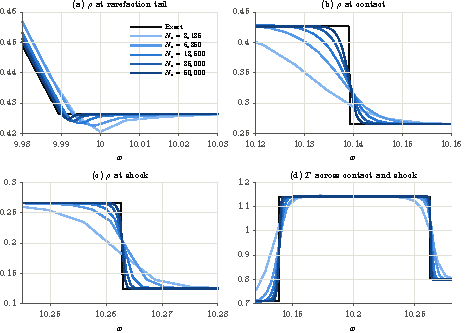
\includegraphics[width=\textwidth]{fig_grid_zoom.pdf}
\caption{Grid refinement at the three waves.  Darker curves are finer grids.  The
shock (c) stays about three cells wide at every resolution.  The contact (b) is
wider in physical units and spans more cells as the grid is refined
(\cref{tab:features}).  The coarse-grid temperature overshoot in (d) disappears by
$N_x=12{,}500$.}
\label{fig:gridzoom}
\end{figure}

\subsection{Grid convergence}
\label{sec:conv_results}

\Cref{tab:L1,tab:L2,tab:orders} and \cref{fig:convergence} give the errors and
observed orders.  Because the solution outside the error window is exact to
round-off, the wave-region $L_2$ errors (\cref{tab:waveL2}) are the global ones
multiplied by $\approx\sqrt{L_x/0.7}=5.35$.  They therefore have identical orders.

\begin{table}[ht]
\centering
\caption{Global $L_1$ errors (mean absolute error over all cells).}
\label{tab:L1}
\small
\begin{tabular}{@{}rcccc@{}}
\toprule
$N_x$ & $\rho$ & $u$ & $p$ & $T$ \\
\midrule
\tabinput{data/tab_conv_L1.tex}
\bottomrule
\end{tabular}
\end{table}

\begin{table}[ht]
\centering
\caption{Global $L_2$ (RMS) errors and temperature peak excess.}
\label{tab:L2}
\small
\begin{tabular}{@{}rccccc@{}}
\toprule
$N_x$ & $\rho$ & $u$ & $p$ & $T$ & $T$ peak excess \\
\midrule
\tabinput{data/tab_conv_L2.tex}
\bottomrule
\end{tabular}
\end{table}

\begin{table}[ht]
\centering
\caption{Wave-region $L_2$ errors, $x\in[x_0-0.3,\ x_0+0.4]$.}
\label{tab:waveL2}
\small
\begin{tabular}{@{}rcccc@{}}
\toprule
$N_x$ & $\rho$ & $u$ & $p$ & $T$ \\
\midrule
\tabinput{data/tab_conv_waveL2.tex}
\bottomrule
\end{tabular}
\end{table}

\begin{table}[ht]
\centering
\caption{Observed orders.  Columns 2--5: pairwise $L_2$ orders~\eqref{eq:order} between
successive grids.  Then the least-squares $L_2$ order over all five grids, the
least-squares $L_1$ order, and the least-squares wave-region $L_2$ order.}
\label{tab:orders}
\small
\begin{tabular}{@{}lccccccc@{}}
\toprule
 & \multicolumn{4}{c}{pairwise $L_2$ order} & \multicolumn{3}{c}{least-squares fit} \\
\cmidrule(lr){2-5}\cmidrule(l){6-8}
 & $3125{\to}6250$ & $6250{\to}12.5$k & $12.5{\to}25$k & $25{\to}50$k & $L_2$ & $L_1$ & wave $L_2$ \\
\midrule
\tabinput{data/tab_conv_orders.tex}
\bottomrule
\end{tabular}
\end{table}

\begin{figure}[ht]
\centering
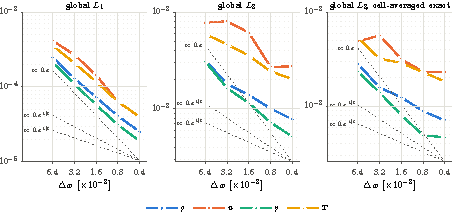
\includegraphics[width=\textwidth]{fig_convergence.pdf}
\caption{Convergence of the global $L_1$ and $L_2$ errors, with the $L_2$ error also
measured against the cell-averaged exact solution (right).  Dotted lines are
reference slopes.}
\label{fig:convergence}
\end{figure}

\paragraph{Interpretation.}  All four variables converge.  The least-squares $L_1$
orders are $0.81$--$0.89$, between the contact value $\tfrac23$ and the shock value
$1$ predicted in \cref{sec:expected_rates}.  For the variables that jump across the
contact ($\rho$, $T$) and for $u$, the $L_2$ orders are $0.40$--$0.49$, between the
contact value $\tfrac13$ and the shock value $\tfrac12$.  Pressure, which does not
jump at the contact, converges at $0.63$, somewhat above $\tfrac12$, because its
faster-converging rarefaction error still makes up a visible share of the total.  The ratio of the $L_2$ order to the $L_1$ order lies between $0.50$ and
$0.72$, close to the value of one half predicted by~\eqref{eq:L1L2delta}.  Temperature, which carries the largest relative contact jump, converges
slowest.  No pairwise order approaches two; the solution is not
smooth, and formal second-order accuracy cannot be verified on this test.

\subsection{Error by wave: which feature limits convergence}
\label{sec:features}

The global squared error is the sum of the contributions of the rarefaction, the
contact and the shock.  \Cref{fig:features} separates them using the zones
$[x_0-0.25,\,x_0+0.07]$, $[x_0+0.07,\,x_0+0.20]$ and $[x_0+0.20,\,x_0+0.40]$.
For density, the least-squares orders of the three contributions are
$\zoneSlopeAA$ (rarefaction), $\zoneSlopeAB$ (contact) and $\zoneSlopeAC$ (shock).
For temperature they are $\zoneSlopeDA$, $\zoneSlopeDB$ and $\zoneSlopeDC$.
The contact is the largest contributor on every grid and has the slowest
convergence, close to the theoretical $\tfrac13$.  It therefore controls the global
$\rho$ and $T$ errors, and its share grows under refinement.

\Cref{tab:features} and \cref{fig:widths} measure this directly.  The shock
thickness stays at $2.9$--$3.1$ cells (physical thickness order
$\shockWidthSlope\approx1$).  This is the self-steepening behaviour of a captured
shock.  The contact thickness scales as $\Delta x^{\contactWidthSlope}$, close to the
$\Delta x^{2/3}$ law for a second-order scheme, so it spans more cells on finer
grids: $4.3$ cells at $N_x=3125$ and $9.3$ cells at $N_x=50{,}000$.  The contact and
shock position errors decrease steadily.  The shock runs about $0.2$ cells ahead of
the exact position, and the contact lags by an amount that decreases faster than
$\Delta x$.

\begin{table}[ht]
\centering
\caption{Measured contact and shock thickness (maximum-gradient definition, from
$\rho$) in physical units and in cells, and the position errors
(numerical minus exact) of the mid-level crossings.}
\label{tab:features}
\small
\begin{tabular}{@{}rcccccc@{}}
\toprule
$N_x$ & $\delta_c$ & $\delta_c/\Delta x$ & $\delta_s$ & $\delta_s/\Delta x$ & contact position error & shock position error \\
\midrule
\tabinput{data/tab_features.tex}
\bottomrule
\end{tabular}
\end{table}

\begin{figure}[ht]
\centering
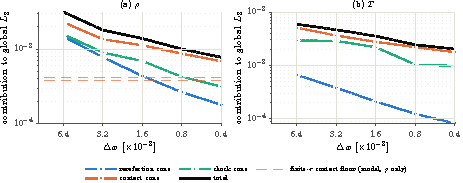
\includegraphics[width=\textwidth]{fig_feature_errors.pdf}
\caption{Contribution of each wave to the global $L_2$ error for (a) density and
(b) temperature.  The dashed band in (a) is the finite-$\tau$ contact floor
predicted by~\eqref{eq:erf_l2}.}
\label{fig:features}
\end{figure}

\begin{figure}[ht]
\centering
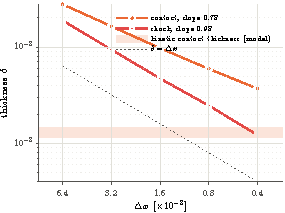
\includegraphics[width=0.62\textwidth]{fig_feature_widths.pdf}
\caption{Measured contact and shock thickness versus grid spacing.  The shaded band
is the kinetic contact thickness~\eqref{eq:dkin} predicted for
$\tau = 5\times10^{-6}$.}
\label{fig:widths}
\end{figure}

\subsection{The velocity error and the sub-cell position of the shock}
\label{sec:phase}

Velocity is the one variable whose $L_2$ error does not decrease monotonically:
$L_2(u)$ rises slightly from $N_x=3125$ to $6250$ and is flat from $25{,}000$ to
$50{,}000$ (\cref{tab:L2}).  This matches the ``velocity stops improving'' observation
recorded in earlier studies.  The zone decomposition shows why.  Between $93\%$
(coarsest grid) and $99\%$ (finest grid) of $L_2(u)^2$ comes from the $\pm4$ cells
around the shock, where $u$ jumps by $u^*=0.93$.  The velocity is continuous across
the contact, and the rarefaction contribution is four to ten times smaller than
the shock contribution.

The contribution from the handful of cells that straddle the shock depends on
\emph{where the exact shock falls inside a cell}.  The metric compares cell values
with the exact solution sampled at cell centres.  A shock near a face therefore
produces one cell with an almost full-jump error, while a shock near a cell centre
splits the error between two cells.  With the exact shock at
$x_s = x_0 + 0.262823$, its fractional position within its cell is
$0.57$, $0.13$, $0.26$, $0.53$ and $0.06$ on the five grids (\cref{tab:phase}).
Grouping the grids by this phase removes the irregularity.  Between the two
mid-cell grids ($N_x=3125$ and $25{,}000$) the shock-zone $L_2(u)$ converges with
order $\shockPhaseSlopeA$.  Between the two near-face grids ($6250$ and $50{,}000$)
the order is $\shockPhaseSlopeB$.  Both match the theoretical $\tfrac12$ for a captured
shock (\cref{fig:phase}a).  The flat $25{,}000\to50{,}000$ velocity result is
therefore a sampling artefact of comparing a point-sampled discontinuous reference
with an $\ord(1)$-per-cell error.  It does not indicate a relaxation-time or
time-step limit.

Averaging the exact solution over each cell, which is the natural reference for a
finite-volume method, reduces the coarse-grid velocity error.  It does not remove
the phase dependence (\cref{fig:phase}b, \cref{tab:orders_avg}), because the discrete
shock profile itself depends on the shock's sub-cell position.  Two practical
consequences follow.  First, $L_1(u)$, which weights the few shock cells less
heavily, converges monotonically with order $0.89$ and is the more robust velocity
metric.  Second, velocity $L_2$ orders should be quoted from least-squares fits over
several grids, preferably with refinement ratios that sample different shock phases,
rather than from a single pair of grids.

\begin{table}[ht]
\centering
\caption{Sub-cell position (phase) of the exact shock, the shock-zone ($\pm4\Delta x$)
velocity error, and that error scaled by $\Delta x^{1/2}$, against point-sampled and
cell-averaged exact solutions.  A phase-independent error would give a constant
scaled value.}
\label{tab:phase}
\small
\begin{tabular}{@{}rccccc@{}}
\toprule
 & & \multicolumn{2}{c}{point-sampled exact} & \multicolumn{2}{c}{cell-averaged exact} \\
\cmidrule(lr){3-4}\cmidrule(l){5-6}
$N_x$ & phase & shock-zone $L_2(u)$ & $/\Delta x^{1/2}$ & shock-zone $L_2(u)$ & $/\Delta x^{1/2}$ \\
\midrule
\tabinput{data/tab_shock_phase.tex}
\bottomrule
\end{tabular}
\end{table}

\begin{table}[ht]
\centering
\caption{Global $L_2$ errors against the cell-averaged exact solution, with pairwise
and least-squares orders (the last column is the least-squares $L_1$ order).}
\label{tab:orders_avg}
\small
\begin{tabular}{@{}rcccc@{}}
\toprule
$N_x$ & $\rho$ & $u$ & $p$ & $T$ \\
\midrule
\tabinput{data/tab_conv_L2avg.tex}
\bottomrule
\end{tabular}\\[6pt]
\begin{tabular}{@{}lcccccc@{}}
\toprule
 & $3125{\to}6250$ & $6250{\to}12.5$k & $12.5{\to}25$k & $25{\to}50$k & $L_2$ fit & $L_1$ fit \\
\midrule
\tabinput{data/tab_conv_orders_avg.tex}
\bottomrule
\end{tabular}
\end{table}

\begin{figure}[ht]
\centering
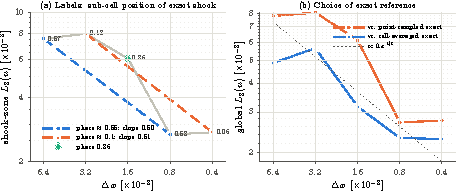
\includegraphics[width=\textwidth]{fig_shock_phase.pdf}
\caption{(a) Shock-zone velocity error.  Point labels give the sub-cell position of
the exact shock.  Grids with matching phase converge at order $\approx\tfrac12$.
(b) Global $L_2(u)$ against point-sampled and cell-averaged exact solutions.}
\label{fig:phase}
\end{figure}

\subsection{The role of the finite relaxation time}
\label{sec:tau_results}

\Cref{sec:contact_diffusion} predicts that at fixed $\tau$ the contact cannot become
thinner than $\delta_c^{\mathrm{kin}} = \kinContactMin$--$\kinContactMax$ for
$\tau=5\times10^{-6}$.  The contact error therefore has a floor of
$\rhoFloorMin$--$\rhoFloorMax$ in global $L_2(\rho)$.  The measured contact thickness
on the finest grid is $3.7\times10^{-3}$, about three times the kinetic value
(\cref{fig:widths}), and the contact-zone density error ($6.8\times10^{-4}$) is still
above the floor (\cref{fig:features}a).  The present study is therefore
discretization-dominated.  Extrapolating the measured $\Delta x^{0.73}$ contact
thickness, the numerical and kinetic thicknesses become equal near
$\Delta x\approx1\times10^{-4}$ ($N_x\approx2\times10^5$).  Below that spacing, further
refinement at $\tau=5\times10^{-6}$ would stop reducing the $\rho$ and $T$ errors.

For the earlier setting $\tau = 5\times10^{-5}$ the kinetic contact is
$10^{1/2}\approx3.2$ times thicker ($3.7$--$4.6\times10^{-3}$).  That is already equal
to the numerical contact thickness at $N_x = 50{,}000$.  This explains the plateau
recorded in the project handoff for that setting (\cref{tab:tau_compare}):
$L_2(\rho)$ was $1.130\times10^{-3}$ at $N_x=40{,}000$ and $1.132\times10^{-3}$ at
$50{,}000$, whereas at $\tau=5\times10^{-6}$ the error keeps falling to
$7.77\times10^{-4}$.  The earlier runs also used a ten times larger time step
($\Delta t = 1.25\times10^{-5}$, CFL $=0.10$), so the comparison does not separate
$\tau$ from $\Delta t$.  It is, however, quantitatively consistent with the
finite-$\tau$ contact floor.

\begin{table}[ht]
\centering
\caption{Global $L_2(\rho)$ at the two relaxation times.  The $\tau=5\times10^{-5}$ values
are the September 13 results recorded in the project handoff (CFL $=0.10$,
$\Delta t=1.25\times10^{-5}$).  The $N_x=50{,}000$ value at that $\tau$ comes from the
separate follow-on run in the same record.}
\label{tab:tau_compare}
\small
\begin{tabular}{@{}rccc@{}}
\toprule
$N_x$ & $\tau=5\times10^{-5}$ (handoff) & $\tau=5\times10^{-6}$ (this study) & ratio \\
\midrule
3,125  & $3.244\times10^{-3}$ & $3.163\times10^{-3}$ & $0.97$ \\
6,250  & $1.961\times10^{-3}$ & $1.806\times10^{-3}$ & $0.92$ \\
12,500 & $1.594\times10^{-3}$ & $1.392\times10^{-3}$ & $0.87$ \\
25,000 & $1.258\times10^{-3}$ & $1.003\times10^{-3}$ & $0.80$ \\
40,000 & $1.130\times10^{-3}$ & --- & --- \\
50,000 & $1.132\times10^{-3}$ & $7.766\times10^{-4}$ & $0.69$ \\
\bottomrule
\end{tabular}
\end{table}

\subsection{Limiter comparison}
\label{sec:limiter_results}

\Cref{tab:limiters} and \cref{fig:limiters} compare the five limiters developed
during the project at $N_x=6250$, under identical physics, $\Delta t$, grid and final
time.  The generalized-minmod case reproduces the convergence-study run at the same
grid to all printed digits, which cross-checks the two independently written
implementations.

\begin{table}[ht]
\centering
\caption{Limiter comparison, $N_x=6250$, $\tau=5\times10^{-6}$, CFL $=0.025$.}
\label{tab:limiters}
\footnotesize
\setlength{\tabcolsep}{4pt}
\begin{tabular}{@{}lcccccc@{}}
\toprule
Limiter & $L_1(\rho)$ & $L_1(u)$ & $L_1(p)$ & $L_1(T)$ & wave $L_1(T)$ & $T$ peak excess \\
\midrule
\tabinput{data/tab_limiters.tex}
\bottomrule
\end{tabular}
\end{table}

\begin{figure}[ht]
\centering
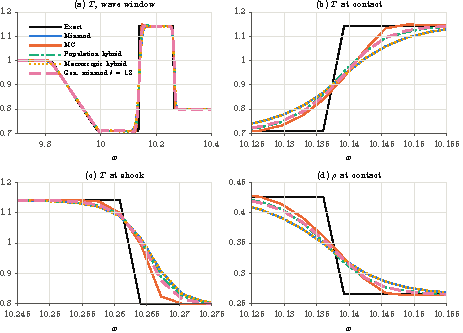
\includegraphics[width=\textwidth]{fig_limiters.pdf}
\caption{Limiter comparison at $N_x=6250$.  Minmod and the macroscopic hybrid nearly
coincide.  MC is the sharpest and shows the largest temperature overshoot, just
behind the contact (b).}
\label{fig:limiters}
\end{figure}

The results reproduce, at the new $\tau$ and CFL, the tradeoff identified earlier in
the project:
\begin{itemize}
  \item MC gives the smallest average errors but the largest temperature peak
        excess ($6.7\times10^{-3}$).  Its compressive slopes, $\phi$ up to $2$,
        overshoot at the contact, and the high-sensitivity populations of
        \cref{tab:sensitivity} amplify the overshoot into $T$.
  \item Minmod has the smallest overshoot ($4.5\times10^{-4}$) but the largest
        average errors.
  \item The macroscopic hybrid behaves almost exactly like minmod.  Its shared
        troubled-cell mask evidently covers most of the cells in which minmod and MC
        would differ, so it rarely uses the MC slope where it matters.
  \item Generalized minmod with $\theta=1.2$ reduces all four global $L_1$ errors by
        $20$--$23\%$ relative to minmod, and reduces MC's temperature peak excess by
        $77\%$.
\end{itemize}

\subsection{The $\theta$ sweep}
\label{sec:theta_results}

\Cref{tab:theta,fig:theta} show the whole family from $\theta=1$ (identical to
minmod) to $\theta=2$ (identical to MC).  The average error decreases monotonically
with $\theta$, and the temperature peak excess increases monotonically.  The family
therefore traces a single diffusion--overshoot tradeoff curve (\cref{fig:theta}b).
No $\theta$ is best on both metrics.  Measured along that curve, $\theta=1.2$ captures
$59\%$ of the $L_1(T)$ reduction available between minmod and MC while incurring
$18\%$ of the overshoot increase.  For comparison, $\theta=1.1$ gives $35\%/7\%$ and
$\theta=1.3$ gives $74\%/30\%$.  $\theta=1.2$ is thus a reasonable compromise, not an
optimum.  The appropriate value depends on how peak temperature error is weighed
against average error.  On the convergence grids the peak excess at $\theta=1.2$
vanishes for $N_x\ge12{,}500$ (\cref{tab:L2}), so the overshoot cost is a
coarse-grid effect at this $\tau$.  No fallback or retry occurred for any $\theta$.

\begin{table}[ht]
\centering
\caption{$\theta$ sweep, $N_x=6250$, $\tau=5\times10^{-6}$, CFL $=0.025$.  The last column
counts limiter fallbacks.}
\label{tab:theta}
\small
\begin{tabular}{@{}lccccccc@{}}
\toprule
$\theta$ & $L_1(\rho)$ & $L_1(u)$ & $L_1(p)$ & $L_1(T)$ & wave $L_1(T)$ & $T$ peak excess & fb \\
\midrule
\tabinput{data/tab_theta.tex}
\bottomrule
\end{tabular}
\end{table}

\begin{figure}[ht]
\centering
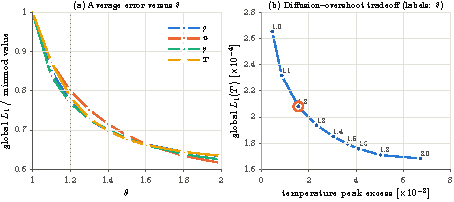
\includegraphics[width=\textwidth]{fig_theta_sweep.pdf}
\caption{(a) Global $L_1$ errors normalized by the minmod ($\theta=1$) values.
(b) Temperature $L_1$ error versus temperature peak excess.  Each point is one
$\theta$; the solver's $\theta=1.2$ is circled.}
\label{fig:theta}
\end{figure}


% ===========================================================================
\section{Summary}
\label{sec:summary}
% ===========================================================================

\subsection{How the solver works, in one paragraph}
The solver replaces the Euler equations with five linear advection equations, one
per discrete velocity $c_i\in\{0,\pm1,\pm3\}$, coupled only through a local BGK
relaxation toward the KT-D1V5 equilibrium.  That equilibrium is the unique
five-population state whose moments reproduce the density, momentum and energy and
the two Euler fluxes (\cref{prop:feq}).  Mass, momentum and energy are carried
exactly by the collision operator and conservatively by the finite-volume
transport.  Each population is upwinded exactly, since upwinding is the Riemann
solution for linear advection.  Accuracy comes from a MUSCL reconstruction whose
slope is limited by the generalized minmod, which is TVD for each population's
transport when $1\le\theta\le2$ (\cref{prop:tvd}).  SSP-RK3 advances everything with a
time step set by the relaxation time, $\Delta t=\tau/4$.  This step resolves the
BGK decay (stiffness exactly $1/\tau$) and keeps the transport Courant number below
$0.01$ on every grid.

\subsection{Principal findings}
\begin{enumerate}
  \item \textbf{Model.}  The KT-D1V5 model reproduces the Euler equations exactly at
        leading order.  Its $\ord(\tau)$ terms are not Navier--Stokes: the viscosity is
        about $3.5$ times the BGK value, the dissipation is not Galilean invariant,
        and there is a spurious density-gradient energy flux (\cref{tab:ce_compare}).
        $\tau$ should be regarded as a regularization that vanishes in the Euler limit.
  \item \textbf{Contact physics of the model.}  A contact moving at speed $U$ diffuses
        with $D_c=\tau(v_1^2-U^2)(v_2^2-U^2)/[(b+2)T]$.  At the Sod contact this is
        eight times weaker than at rest, and it would become anti-diffusive for
        $|U|>v_1$.  At the level of this first-order analysis, the result limits the flow speeds
        for which the present velocity set is usable.
  \item \textbf{Temperature sensitivity.}  $\partial T/\partial f_i = [(c_i-u)^2+\eta_i^2-bT]/(b\rho)$
        reaches about $7$ for the fast counter-moving population in the post-shock
        state.  This explains why limiter-induced overshoot appears first, and most
        strongly, in $T$.
  \item \textbf{Convergence.}  With $\tau=5\times10^{-6}$ and $\mathrm{CFL}=0.025$ on five
        grids up to $N_x=50{,}000$, all runs were clean (no retries, fallbacks or
        repairs) and conservative to round-off.  The fitted orders are
        $L_1\approx0.81$--$0.89$ and $L_2\approx0.40$--$0.63$, which is the correct
        behaviour for a second-order method on a solution with a shock and a
        contact.  The contact is the slowest-converging feature
        (thickness $\propto\Delta x^{0.73}$, close to the theoretical $\Delta x^{2/3}$).
        The shock stays three cells wide.
  \item \textbf{Velocity anomaly explained.}  The non-monotone $L_2(u)$ comes from the
        sub-cell position of the exact shock relative to the grid.  Grids with
        matching phase converge at order $0.50$--$0.51$.  $L_1(u)$ converges
        monotonically.
  \item \textbf{Relaxation time.}  At $\tau=5\times10^{-6}$ the grids used here remain
        discretization-dominated.  The kinetic contact floor is predicted to matter
        only near $N_x\approx2\times10^5$.  At $\tau=5\times10^{-5}$ the floor is reached
        near $N_x\approx5\times10^4$, consistent with the plateau seen in the earlier
        study.
  \item \textbf{Limiter.}  $\theta=1.2$ lowers every global $L_1$ error by $20$--$23\%$
        relative to minmod and cuts MC's temperature overshoot by $77\%$.  The
        $\theta$ sweep shows a single monotone tradeoff: $\theta=1.2$ buys $59\%$ of the
        attainable $L_1(T)$ improvement for $18\%$ of the overshoot cost.  It is a
        defensible compromise, not a unique optimum.
\end{enumerate}

\subsection{Limitations and recommended next steps}
\begin{itemize}
  \item Every convergence run used the same $\Delta t$, so temporal error was not
        measured.  A short $\Delta t$-halving test at $N_x=50{,}000$ would confirm the
        expectation that it is negligible.
  \item Formal second-order accuracy should be verified on a smooth problem (for
        example an isentropic or small-amplitude acoustic pulse), because Sod
        cannot show it.
  \item The finite-$\tau$ floor analysis is a first-order Chapman--Enskog estimate.
        A $\tau$ study at fixed $\Delta t$ and a fine grid would test it directly.
  \item Velocity convergence should be reported from $L_1$ norms or from phase-varied
        grid sequences, to avoid the shock-phase artefact.
  \item The contact-diffusion result implies that a two-dimensional extension needs
        a velocity set whose slowest speed exceeds the expected flow speeds, or a
        higher-order (Navier--Stokes-level) equilibrium~\citep{KataokaTsutahara2004NS,Gan2018}.
\end{itemize}


% ===========================================================================
\appendix
\section{Reproducibility}
\label{app:repro}
% ===========================================================================
All numbers and figures in \cref{sec:results} are generated by scripts in the
research folder:
\begin{itemize}
  \item \file{run_d1v5_gminmod_L2_convergence.m}: five-grid study.  Each grid
        is cached in \texttt{results/runs/} with $\theta$, $\tau$, CFL and $N_x$ in the
        file name.  \file{run_d1v5_gminmod_L2_convergence(Nx)} runs a single
        grid, which allows several grids to run in parallel.
  \item \file{d1v5_sodshock_limiter_history_comparison.m}: five-limiter
        comparison at $N_x=6250$, $\tau=5\times10^{-6}$, $\mathrm{CFL}=0.025$.
  \item \file{report_d1v5_math/scripts/run_d1v5_theta_sweep.m}: $\theta$ sweep
        using the unmodified solver.
  \item \file{report_d1v5_math/scripts/verify_kt_d1v5_theory.m}: numerical
        checks of every analytical result in \cref{sec:model,sec:ce_discrete}.
  \item \file{report_d1v5_math/scripts/make_theory_figures.m} and
        \file{make_results_figures.m}: all figures and the tables
        in \cref{sec:results}.
\end{itemize}
The earlier $\tau=5\times10^{-5}$ and $\tau=5\times10^{-6}$/CFL $=0.05$ result files are
preserved unchanged in \file{results/backup_2026-09-16_tau5e-6_study/}.

% ===========================================================================
\begin{thebibliography}{99}
\small

\bibitem{BGK1954}
P.~L. Bhatnagar, E.~P. Gross, and M.~Krook,
``A model for collision processes in gases. I. Small amplitude processes in charged and neutral one-component systems,''
\emph{Physical Review} \textbf{94}(3), 511--525 (1954).
\href{https://doi.org/10.1103/PhysRev.94.511}{doi:10.1103/PhysRev.94.511}

\bibitem{BrennerThomeeWahlbin1975}
P.~Brenner, V.~Thom\'ee, and L.~B. Wahlbin,
\emph{Besov Spaces and Applications to Difference Methods for Initial Value Problems},
Lecture Notes in Mathematics, vol.~434, Springer (1975).
\href{https://doi.org/10.1007/BFb0068125}{doi:10.1007/BFb0068125}

\bibitem{Cercignani1988}
C.~Cercignani,
\emph{The Boltzmann Equation and Its Applications},
Applied Mathematical Sciences, vol.~67, Springer (1988).
\href{https://doi.org/10.1007/978-1-4612-1039-9}{doi:10.1007/978-1-4612-1039-9}

\bibitem{ChapmanCowling1970}
S.~Chapman and T.~G. Cowling,
\emph{The Mathematical Theory of Non-uniform Gases}, 3rd ed.,
Cambridge University Press (1970).

\bibitem{Gan2018}
Y.~Gan, A.~Xu, G.~Zhang, and H.~Lai,
``Three-dimensional discrete Boltzmann models for compressible flows in and out of equilibrium,''
\emph{Proceedings of the Institution of Mechanical Engineers, Part C: Journal of Mechanical Engineering Science}
\textbf{232}(3), 477--490 (2018).
\href{https://doi.org/10.1177/0954406217742181}{doi:10.1177/0954406217742181}

\bibitem{Gottlieb2001}
S.~Gottlieb, C.-W. Shu, and E.~Tadmor,
``Strong stability-preserving high-order time discretization methods,''
\emph{SIAM Review} \textbf{43}(1), 89--112 (2001).
\href{https://doi.org/10.1137/S003614450036757X}{doi:10.1137/S003614450036757X}

\bibitem{Harten1977}
A.~Harten,
``The artificial compression method for computation of shocks and contact discontinuities. I. Single conservation laws,''
\emph{Communications on Pure and Applied Mathematics} \textbf{30}(5), 611--638 (1977).
\href{https://doi.org/10.1002/cpa.3160300506}{doi:10.1002/cpa.3160300506}

\bibitem{Harten1983}
A.~Harten,
``High resolution schemes for hyperbolic conservation laws,''
\emph{Journal of Computational Physics} \textbf{49}(3), 357--393 (1983).
\href{https://doi.org/10.1016/0021-9991(83)90136-5}{doi:10.1016/0021-9991(83)90136-5}

\bibitem{KataokaTsutahara2004Euler}
T.~Kataoka and M.~Tsutahara,
``Lattice Boltzmann method for the compressible Euler equations,''
\emph{Physical Review E} \textbf{69}, 056702 (2004).
\href{https://doi.org/10.1103/PhysRevE.69.056702}{doi:10.1103/PhysRevE.69.056702}

\bibitem{KataokaTsutahara2004NS}
T.~Kataoka and M.~Tsutahara,
``Lattice Boltzmann model for the compressible Navier--Stokes equations with flexible specific-heat ratio,''
\emph{Physical Review E} \textbf{69}, 035701(R) (2004).
\href{https://doi.org/10.1103/PhysRevE.69.035701}{doi:10.1103/PhysRevE.69.035701}

\bibitem{KurganovTadmor2000}
A.~Kurganov and E.~Tadmor,
``New high-resolution central schemes for nonlinear conservation laws and convection--diffusion equations,''
\emph{Journal of Computational Physics} \textbf{160}(1), 241--282 (2000).
\href{https://doi.org/10.1006/jcph.2000.6459}{doi:10.1006/jcph.2000.6459}

\bibitem{Kuznetsov1976}
N.~N. Kuznetsov,
``Accuracy of some approximate methods for computing the weak solutions of a first-order quasi-linear equation,''
\emph{USSR Computational Mathematics and Mathematical Physics} \textbf{16}(6), 105--119 (1976).
\href{https://doi.org/10.1016/0041-5553(76)90046-X}{doi:10.1016/0041-5553(76)90046-X}

\bibitem{LeVeque2002}
R.~J. LeVeque,
\emph{Finite Volume Methods for Hyperbolic Problems},
Cambridge University Press (2002).
\href{https://doi.org/10.1017/CBO9780511791253}{doi:10.1017/CBO9780511791253}

\bibitem{MandalDeshpande1994}
J.~C. Mandal and S.~M. Deshpande,
``Kinetic flux vector splitting for Euler equations,''
\emph{Computers \& Fluids} \textbf{23}(2), 447--478 (1994).
\href{https://doi.org/10.1016/0045-7930(94)90050-7}{doi:10.1016/0045-7930(94)90050-7}

\bibitem{OberkampfRoy2010}
W.~L. Oberkampf and C.~J. Roy,
\emph{Verification and Validation in Scientific Computing},
Cambridge University Press (2010).
\href{https://doi.org/10.1017/CBO9780511760396}{doi:10.1017/CBO9780511760396}

\bibitem{Roache1998}
P.~J. Roache,
\emph{Verification and Validation in Computational Science and Engineering},
Hermosa Publishers, Albuquerque (1998).

\bibitem{Shan2006}
X.~Shan, X.-F. Yuan, and H.~Chen,
``Kinetic theory representation of hydrodynamics: a way beyond the Navier--Stokes equation,''
\emph{Journal of Fluid Mechanics} \textbf{550}, 413--441 (2006).
\href{https://doi.org/10.1017/S0022112005008153}{doi:10.1017/S0022112005008153}

\bibitem{ShuOsher1988}
C.-W. Shu and S.~Osher,
``Efficient implementation of essentially non-oscillatory shock-capturing schemes,''
\emph{Journal of Computational Physics} \textbf{77}(2), 439--471 (1988).
\href{https://doi.org/10.1016/0021-9991(88)90177-5}{doi:10.1016/0021-9991(88)90177-5}

\bibitem{Sod1978}
G.~A. Sod,
``A survey of several finite difference methods for systems of nonlinear hyperbolic conservation laws,''
\emph{Journal of Computational Physics} \textbf{27}(1), 1--31 (1978).
\href{https://doi.org/10.1016/0021-9991(78)90023-2}{doi:10.1016/0021-9991(78)90023-2}

\bibitem{Sweby1984}
P.~K. Sweby,
``High resolution schemes using flux limiters for hyperbolic conservation laws,''
\emph{SIAM Journal on Numerical Analysis} \textbf{21}(5), 995--1011 (1984).
\href{https://doi.org/10.1137/0721062}{doi:10.1137/0721062}

\bibitem{Toro2009}
E.~F. Toro,
\emph{Riemann Solvers and Numerical Methods for Fluid Dynamics: A Practical Introduction}, 3rd ed.,
Springer (2009).
\href{https://doi.org/10.1007/b79761}{doi:10.1007/b79761}

\bibitem{vanLeer1977}
B.~van Leer,
``Towards the ultimate conservative difference scheme. IV. A new approach to numerical convection,''
\emph{Journal of Computational Physics} \textbf{23}(3), 276--299 (1977).
\href{https://doi.org/10.1016/0021-9991(77)90095-X}{doi:10.1016/0021-9991(77)90095-X}

\bibitem{vanLeer1979}
B.~van Leer,
``Towards the ultimate conservative difference scheme. V. A second-order sequel to Godunov's method,''
\emph{Journal of Computational Physics} \textbf{32}(1), 101--136 (1979).
\href{https://doi.org/10.1016/0021-9991(79)90145-1}{doi:10.1016/0021-9991(79)90145-1}

\bibitem{WarmingHyett1974}
R.~F. Warming and B.~J. Hyett,
``The modified equation approach to the stability and accuracy analysis of finite-difference methods,''
\emph{Journal of Computational Physics} \textbf{14}(2), 159--179 (1974).
\href{https://doi.org/10.1016/0021-9991(74)90011-4}{doi:10.1016/0021-9991(74)90011-4}

\bibitem{XuChenCai2021}
L.~Xu, R.~Chen, and X.-C. Cai,
``Parallel finite-volume discrete Boltzmann method for inviscid compressible flows on unstructured grids,''
\emph{Physical Review E} \textbf{103}, 023306 (2021).
\href{https://doi.org/10.1103/PhysRevE.103.023306}{doi:10.1103/PhysRevE.103.023306}

\bibitem{XuZhangZhang2018}
A.~Xu, G.~Zhang, and Y.~Zhang,
``Discrete Boltzmann modeling of compressible flows,''
in \emph{Kinetic Theory}, G.~Z. Kyzas and A.~C. Mitropoulos (eds.), InTech (2018), ch.~2;
\href{https://arxiv.org/abs/1708.09187}{arXiv:1708.09187}.

\end{thebibliography}

\end{document}
